%!TEX root=Principal.tex
\chapter{ESTUDO DE CASO}
\label{cap:estudocaso}
Com o método para construção de projetos de interação humano-robô centrado no usuário especificado no capítulo~\ref{cap:projetoihr}, um estudo de caso é apresentado. O escopo deste estudo de caso envolve a aproximação do robô para o ser humano em um ambiente doméstico simulado. Na etapa do mecanismo de tomada de decisão proposta no método é criado de um classificador Bayesiano para ilustrar essa etapa detalhadamente. As informações das ações do robô e informações de comportamento e percepção do usuário são consumidos para construção do classificador. A classificação do usuário é feita no formato de Personas, conforme proposto no método apresentado por essa tese no capítulo~\ref{cap:projetoihr}. A partir desse escopo é iniciado o desenvolvimento do classificador, a partir da definição das variáveis.

\section{VARIÁVEIS DE OBSERVAÇÃO}
\label{sec:ec_variaveis}
Com base nas variáveis apresentadas na literatura, consolidadas na seção~\ref{sec:variaveis}, foram mapeadas quais estão de acordo com o escopo. Elas devem possuir seus valores limitados para que simplifique as tabelas de probabilidades condicionais do classificador Bayesiano. A tabela~\ref{tab:variaveisvalores} apresenta as variáveis e a restrição do domínio de cada uma. 

\begin{table}[!ht]
	\caption{Variáveis de observação escolhidas}
	\label{tab:variaveisvalores}
	\centering
	\begin{tabular}{c | c}
		\hline
		Variável & Valor \\
		\hline
		Gestos & curto \\
		& longo \\
		\hline
		Estilo da Fala & educada \\
		& autoritária \\
		\hline
		Expressão Facial & amigável \\
		& não amigável \\
		\hline
		Proximidade & longe - (Entre Pública e Social ) \\
		& perto - (Entre Pessoal e Íntima ) \\
		\hline
		Velocidade & rápida \\
		& devagar \\
		\hline
		Posição & sentado \\
		& em pé \\
		\hline
		Conforto & sim \\
		& não \\
		\hline
		Medo & sim \\
		& não \\
		\hline
	\end{tabular}
	\smallcaption{Fonte: O autor.}
\end{table}

As variáveis da tabela~\ref{tab:variaveisvalores} são importantes, pois auxiliam a determinar o comportamento de reação do perfil do usuário para um mesmo tipo de ação do robô. Por exemplo, se o robô encontra-se próximo da pessoa, entre as zonas Pessoal e Íntima, um gesto com o manipulador com grande amplitude pode gerar um desconforto maior, do que o mesmo gesto ocorrendo entre as zonas Pública e Social. Outro cenário é a aproximação do manipulador próximo ao rosto do usuário, a reação é positiva ou negativa.

Alguns exemplos sobre os domínios das variáveis podem auxiliar a compreender quais são as ações correspondentes. Um exemplo para estilo de fala educada e autoritária são: ``Por favor, poderia me auxiliar a encontrar minha garrafa'' e ``Encontre minha garrafa'', respectivamente. Para ilustrar o domínio das expressões faciais é apresentada a figura~\ref{fig:dominioexpressoesfaciais}.

\begin{figure}[ht!]
	\centering
	\begin{minipage}{\textwidth}
		\caption{Exemplos das faces apresentadas pelo robô.}
		\begin{subfigure}[b]{0.48\textwidth}
			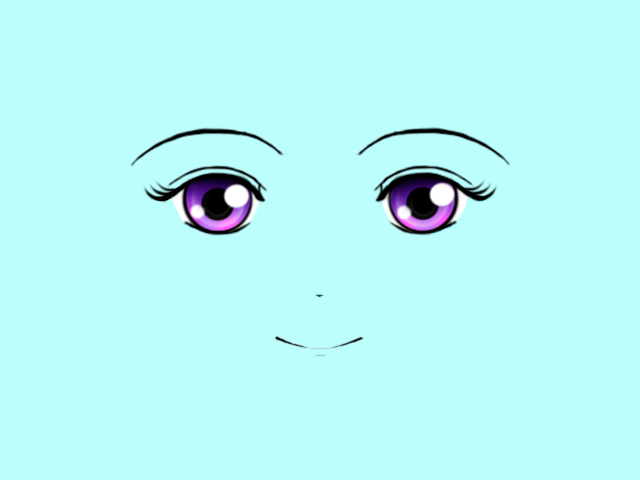
\includegraphics[width=\textwidth]{happy.png}
	        \caption{Feliz}
	        \label{fig:feliz}
	    \end{subfigure}
	    \hfill
		\begin{subfigure}[b]{0.48\textwidth}
	        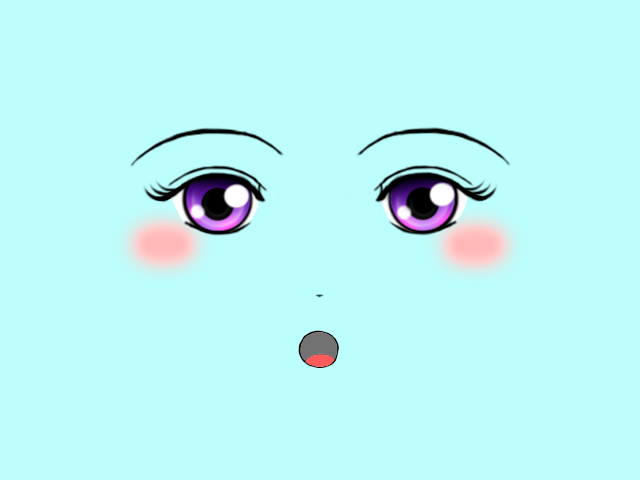
\includegraphics[width=\textwidth]{surprise.png}
	        \caption{Surpresa}
	        \label{fig:surpresa}
	    \end{subfigure}

		\begin{subfigure}[b]{0.48\textwidth}
	        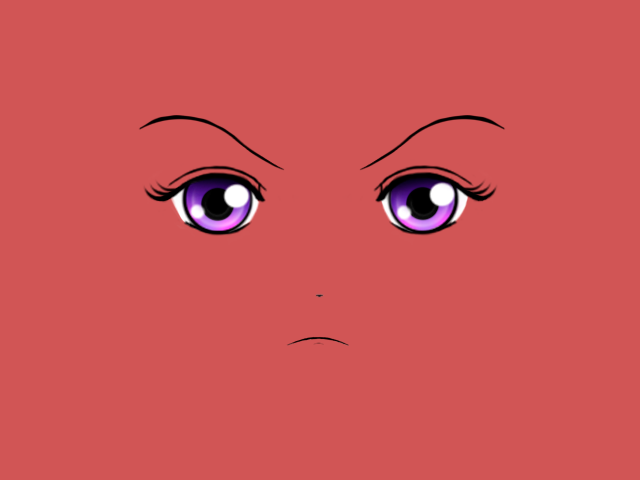
\includegraphics[width=\textwidth]{angry.png}
	        \caption{Nervosa}
	        \label{fig:nervosa}
    	\end{subfigure}
		\hfill
		\begin{subfigure}[b]{0.48\textwidth}
	        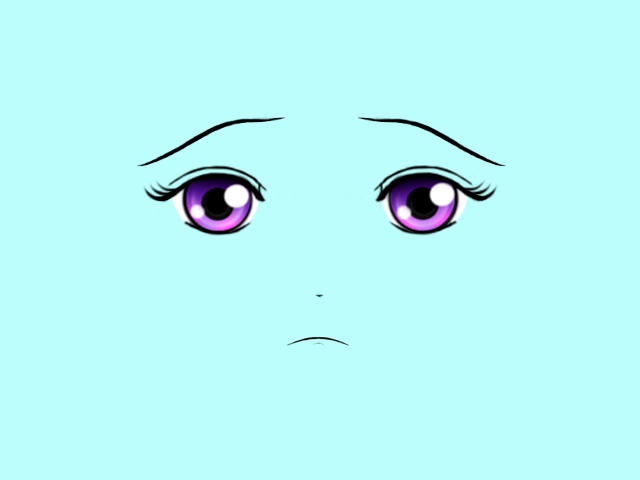
\includegraphics[width=\textwidth]{sad.png}
	        \caption{Triste}
	        \label{fig:triste}
    	\end{subfigure}
		\smallcaption{Fonte: adaptado de \cite{gonbata:2016}.}
		\label{fig:dominioexpressoesfaciais}
	\end{minipage}
\end{figure}

Nos exemplos apresentados na figura~\ref{fig:dominioexpressoesfaciais}, pode-se definir dentro do domínio da variável as figuras \ref{fig:feliz} e \ref{fig:surpresa} como expressões amigáveis e as figuras \ref{fig:nervosa} e \ref{fig:triste} como não amigáveis, dado os sentimentos que essas expressões representam. As variáveis de conforto e medo são obtidas através da declaração do usuário através dos questionários pós teste, apresentado na seção~\ref{sec:questionarioposteste}. Com o domínio das variáveis definidos, o próximo passo é estabelecer o contexto de uso.

\section{CONTEXTO DE USO}
\label{sec:ec_contextouso}
A definição do contexto de uso é baseada em um texto descritivo que delimita todo o cenário da aplicação e como foi planejado o experimento. Esse cenário descreve quem é o usuário, quais os pontos de interação com o sistema, como será o comportamento do usuário e do robô. O contexto descrito delimita todo o escopo do teste. Ele assegura que as observações tenham o objetivo de garantir a qualidade do uso dentro daquele cenário. A figura~\ref{fig:contextouso} apresenta o cenário aplicado no contexto de uso dessa tese.

\begin{figure}[ht!]
	\centering
	\begin{minipage}{\textwidth}
		\caption{Ilustração do contexto de uso}
		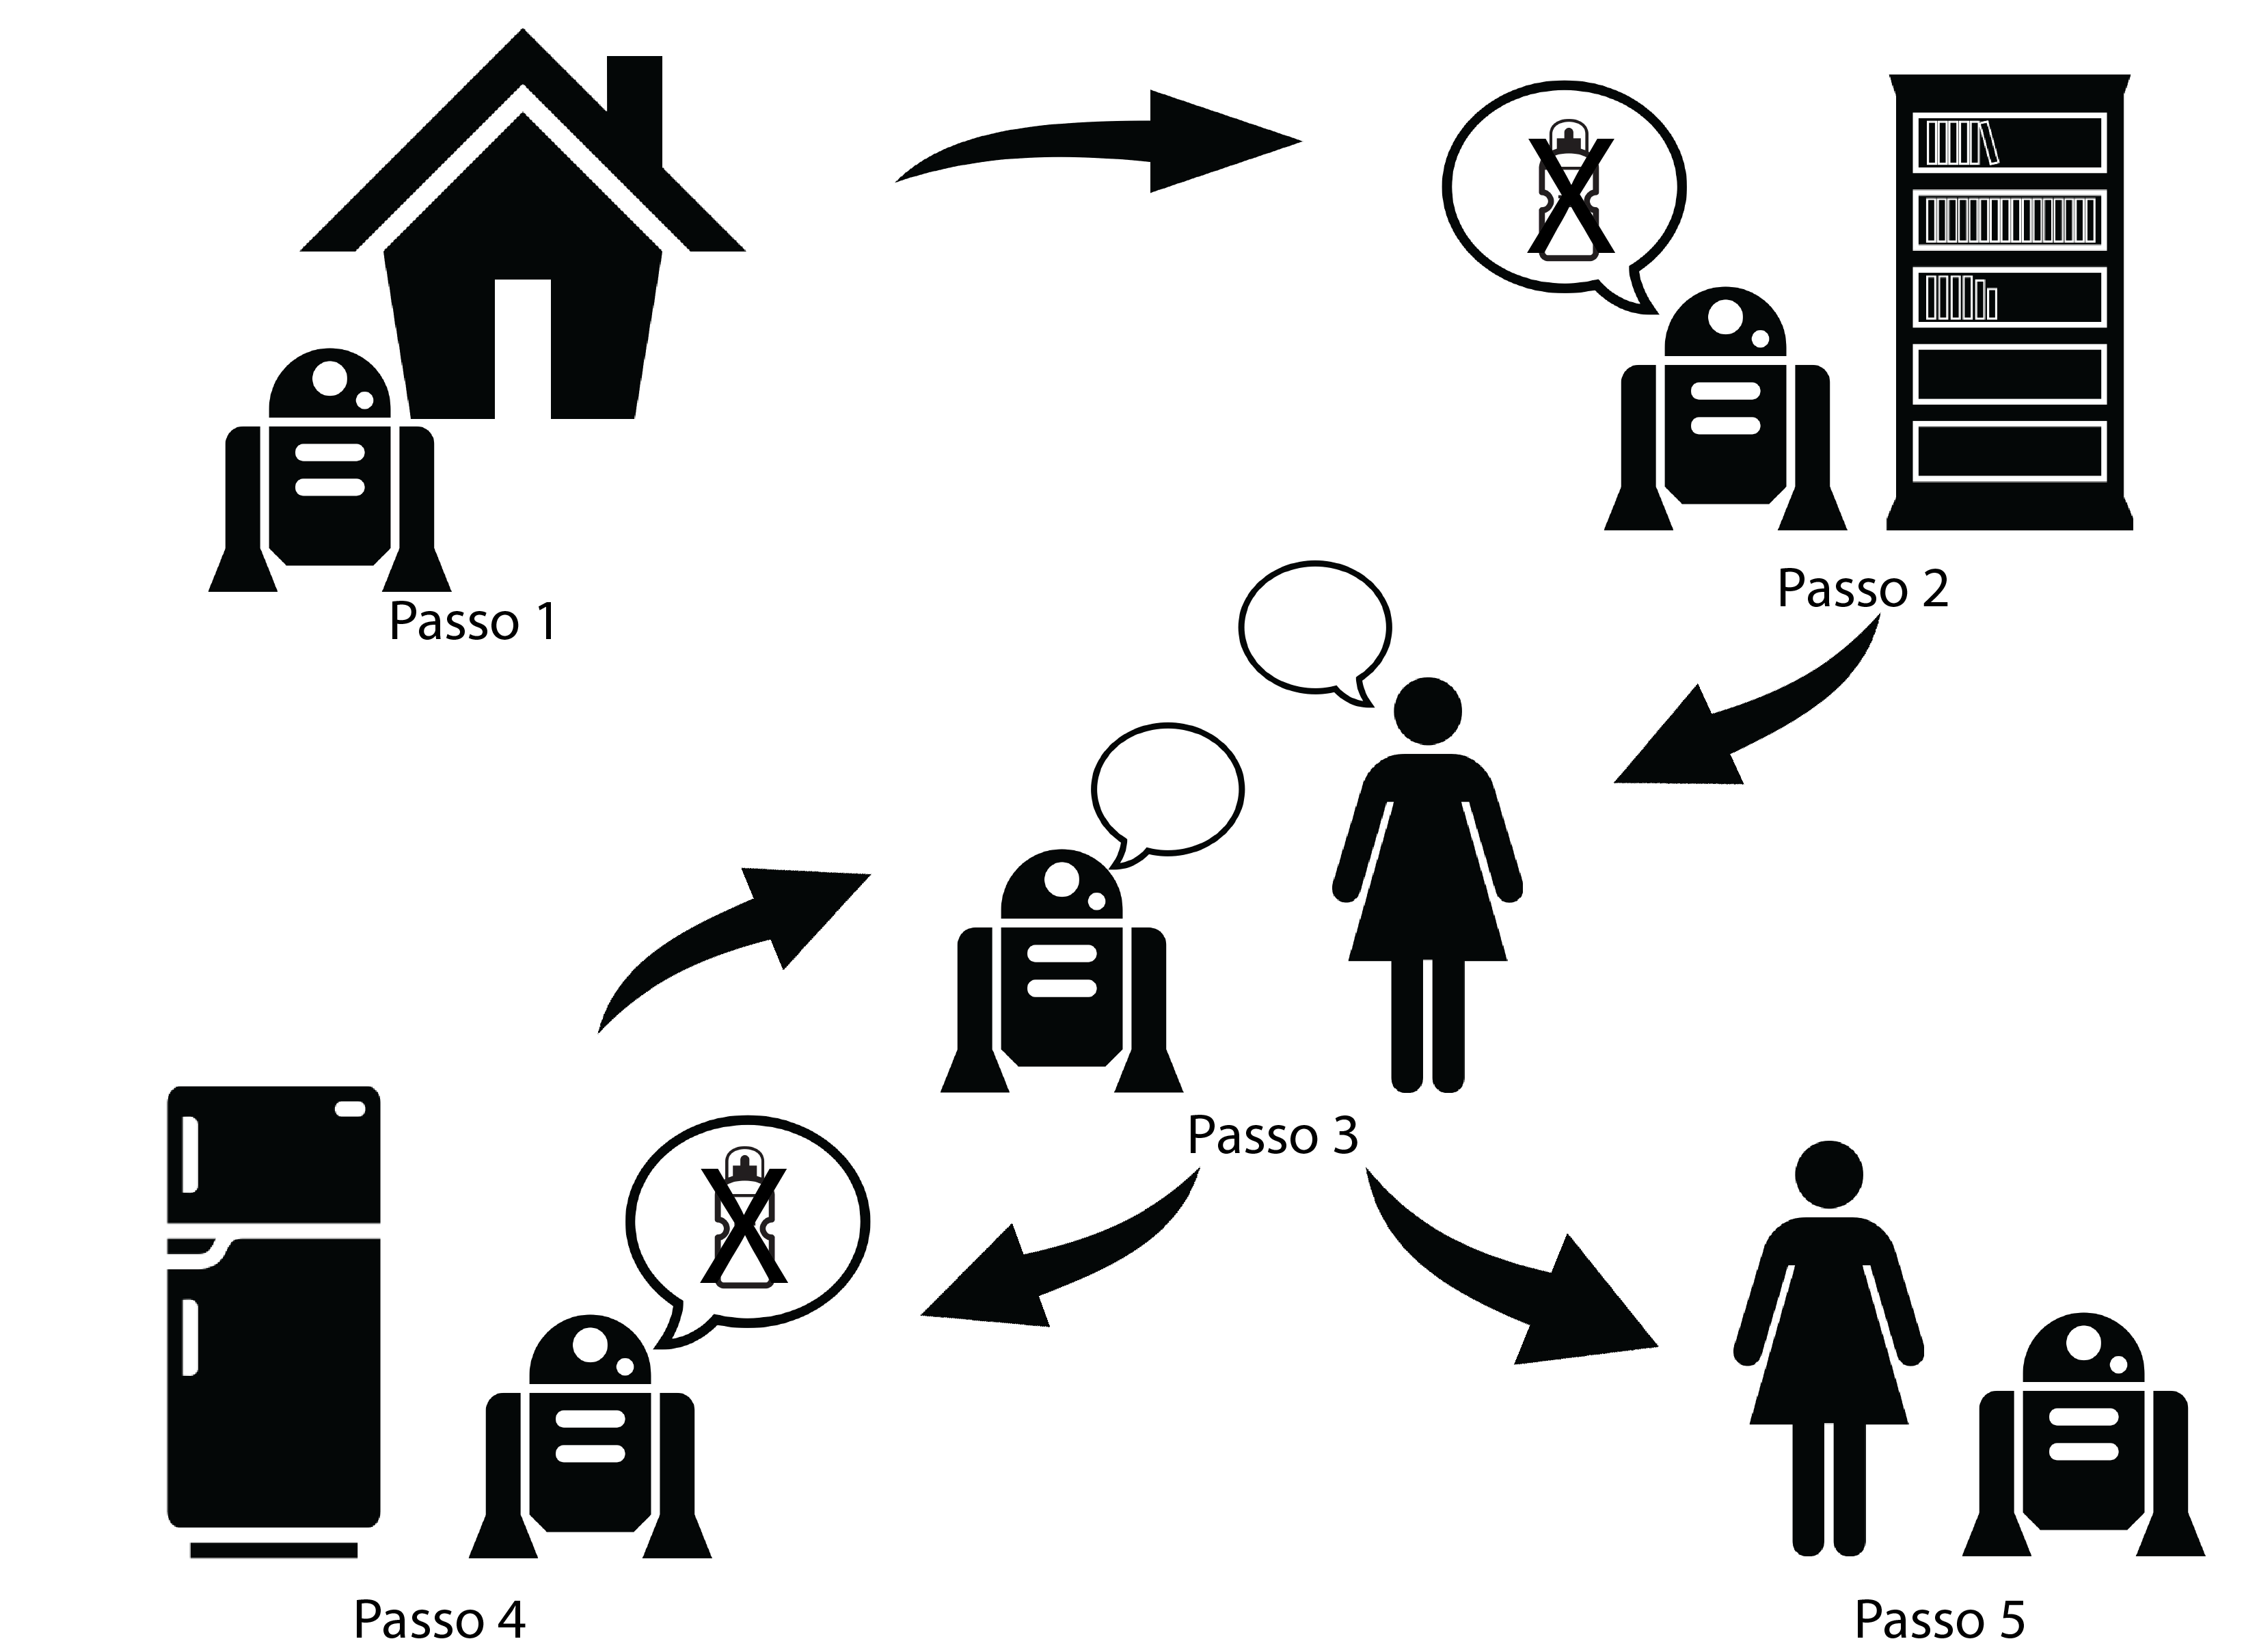
\includegraphics[width=\textwidth]{contexto-uso.png}
		\smallcaption{Fonte: o autor.}
		\label{fig:contextouso}
	\end{minipage}
\end{figure}

O cenário apresentado na figura~\ref{fig:contextouso} ilustra uma situação onde o robô entra em sua casa (passo 1) e vai até a estante onde ele deixou uma garrafa. A garrafa não está mais no local que ele deixou (passo 2), então ele vai até a pessoa que convive com ele no ambiente da casa. Ao interagir com a pessoa, o robô pergunta se ela viu a garrafa e recebe uma resposta negativa (passo 3). Na sequência, o robô procura pela garrafa em outro cômodo da casa, onde também não encontra (passo 4). O robô então retorna ao encontro da pessoa, e solicita a ajuda para procurar pela garrafa (passo 3). Como última etapa, a pessoa atende o pedido e ambos saem para procurar pela garrafa (passo 5), finalizando assim o cenário.

Através dessa ilustração pode-se definir o contexto de uso desta tese, onde o robô realiza a aproximação de pessoas que convivem com ele dentro de uma casa. Essa aproximação é realizada com o objetivo de solicitar ajuda ao humano para encontrar um objeto que foi deixado em algum lugar da casa. Com as variáveis identificadas e o contexto de uso definidos, é necessário realizar a especificação dos questionários de pré e pós teste para saber o que será avaliado dentro do projeto.

\section{QUESTIONÁRIO PRÉ TESTE}
\label{sec:questionariopreteste}
Para apoiar o processo de obtenção das informações e construção dos perfis dos usuários, são utilizados dois questionários. O primeiro, aplicado no momento anterior ao experimento de interação, tem como objetivo mapear as informações referentes às características físicas que tem a possibilidade do robô utilizar sensores para reconhecê-las, adesão a tecnologia, contatos prévios com robôs, questões culturais onde o usuário declara quais locais ele possui mais afinidade e quais ele já teve o privilégio de visitar, além da expectativa de possuir um robô em casa ou no trabalho. As questões são apresentadas na tabela~\ref{tab:questoespreteste}, onde a coluna construção contém os grupos de informações que conferem com a parte do perfil que elas auxiliam a preencher conforme apresentado por \textcite{barbosa:2010} e \textcite{baxter:2015}. Todas as questões a seguir fazem parte do questionário pré-experimento.

\begin{longtable}{ m{7 cm} | m{4cm} | m{4cm} }
	\caption{Questões aplicadas no questionário pré teste }
	\label{tab:questoespreteste} \\	\hline
	Pergunta & Opções & Construção \\ \hline
	Informe seu nome completo & Texto Aberto & Identificação \\ \hline
	e-mail para contato & Texto Aberto & Contato Usuário \\ \hline
	Informe o número do seu celular & Texto Aberto & Contato Usuário \\ \hline
	Testes poderão ocorrer usando o Robô no Centro Universitário FEI. Você gostaria de realizar o teste com o robô físico? & Sim; Não & Contato Usuário \\ \hline
	Qual a sua idade? (em anos) & Numérico & Demográfico \\ \hline
	Qual a sua altura? (em metros) & Numérico & Demográfico \\ \hline
	Informa seu gênero & Feminino; Masculino; Prefiro não dizer & Demográfico \\ \hline
	Na maior parte do tempo, você se considera uma pessoa com feição: & Sorridente; Normal; Séria/Fechada & Social \\ \hline
	Você se considera uma pessoa sociável? & Sim; Não & Social \\ \hline
	Você utiliza óculos de grau? (Obs: Pessoas com lente de contato, por favor, respondam não. A intenção é identificar a armação.) & Sim; Não & Físico \\ \hline
	Você possui cabelo comprido? & Sim; Não & Físico \\ \hline
	Qual etnia você se considera? & Amarela; Branca; Indígena; Parda; Preta; Não declarada & Etnográfico \\ \hline
	Qual(is) dispositivo(s) tecnológico(s) você mais utiliza (marque 1 ou mais opções): & Celular; Computador (de mesa ou notebook); Tablet; Smart TV; Relógio Smart; MP3 Player; Câmera Fotográfica Digital; Leitor de e-Book; outros & Experiência com Tecnologias \\ \hline
	Qual(is) dispositivo(s) tecnológico(s) você nunca utilizou (marque 1 ou mais opções): & Celular; Computador (de mesa ou notebook); Tablet; Smart TV; Relógio Smart; MP3 Player; Câmera Fotográfica Digital; Leitor de e-Book; Já utilizei todas & Experiência com Tecnologias \\ \hline
	Você possui conta em banco digital (ex: Original, Neon, etc.) ? & Sim; Não & Atitudes e Valores \\ \hline
	Você possui cartão de crédito digital (ex: Nubank, Digio, etc.) ? & Sim, Não & Atitudes e Valores \\ \hline
	Qual o principal meio de pagamento de suas contas? & Celular; Computador; Tablet; Autoatendimento; Caixa Físico & Atitudes e Valores \\ \hline
	Você utiliza redes sociais? & Sim; Não & Experiência com Tecnologias \\ \hline
	Quais as redes sociais que você mais utiliza (marque 1 ou mais opções): (Se sim, para a resposta anterior) & Facebook, Instagram, Twitter, Google Plus, Snapchat, outras & Experiência com Tecnologias \\ \hline
	Qual foi o local de nascimento? (Informe da seguinte maneira: Cidade; Estado; País) & Texto Aberto & Cultural \\ \hline
	Em qual local, você viveu por mais tempo durante sua infância e adolescência? (Informe da seguinte maneira: Cidade; Estado; País) & Texto Aberto & Cultural \\ \hline
	Qual o seu atual local de moradia? (Informe da seguinte maneira: Cidade; Estado; País) & Texto Aberto & Cultural \\ \hline
	Qual o país que você melhor se identifica com a cultura? (Considere também a opção do seu país de nascimento.) & Texto Aberto & Cultural \\ \hline
	Qual a cidade, na sua opinião, que melhor representa a cultura que você se identifica (resposta não dependente da questão acima)? & Texto Aberto & Cultural \\ \hline
	Você visitou outros países, além do Brasil? & Sim; Não & Cultural \\ \hline
	Quais países você já visitou? (Responda separando os países por ponto e vírgula, ex: França; Estados Unidos; Itália; Japão;) & Texto Aberto & Cultural \\ \hline
	Aproximadamente, quantas cidades na região nordeste do Brasil você visitou? & Numérico & Cultural \\ \hline
	Aproximadamente, quantas cidades na região norte do Brasil você visitou? & Numérico & Cultural \\ \hline
	Aproximadamente, quantas cidades na região centro-oeste do Brasil você visitou? & Numérico & Cultural \\ \hline
	Aproximadamente, quantas cidades na região sudeste do Brasil você visitou? & Numérico & Cultural \\ \hline
	Aproximadamente, quantas cidades na região sul do Brasil você visitou? & Numérico & Cultural \\ \hline
	Em algum momento de sua vida, você teve contato com robôs? & Sim; Não & Experiência com Produto \\ \hline
	Se sim para a questão anterior, quais tipos de robôs você teve contato (marque 1 ou mais opções): & Parecido com animais, Parecido com pessoas, Robôs de linha de produção/fábrica, Robôs Móveis (que contém rodas), outros  & Experiência com Produto \\ \hline
	O que você espera do comportamento do Robô ao tê-lo em sua casa? & Texto Aberto & Experiência com Produto \\ \hline
	O que você espera do comportamento do Robô ao tê-lo em seu trabalho? & Texto Aberto & Experiência com Produto \\ \hline
	Dadas as questões anteriores, gostaria de fazer mais algum comentário sobre você? & Texto Aberto & Comentários Aberto \\ \hline
	\smallcaption{Fonte: O autor.}
\end{longtable}

A partir das informações coletadas com as questões apresentadas na tabela~\ref{tab:questoespreteste}, é possível determinar o perfil de cultura declarado pelo usuário, informações etnográficas que irão auxiliar na identificação da Persona. Expectativas sobre a interação com robôs em ambientes domésticos e profissionais, também são adquiridas. Essas informações auxiliam a determinar o ponto de partida para a análise e criação das personas discutidas no capítulo~\ref{cap:projetoihr}.

\section{QUESTIONÁRIO PÓS TESTE}
\label{sec:questionarioposteste}
O questionário pós teste mantém o foco na interação do usuário que ocorreu durante o experimento e quais pontos do robô mais agradaram em sua opinião. Além disso, um detalhe sobre a posição do usuário durante o experimento (sentado ou em pé) é coletada, pois esta informação pode influenciar na interação com o robô. As questões apresentas na tabela~\ref{tab:questoesposteste}, a seguir, compõe o questionário pós-teste.

\begin{longtable}{ m{7 cm} | m{4cm} | m{4cm} }
	\caption{Questões aplicadas no questionário pós teste }
	\label{tab:questoesposteste} \\	\hline
	Pergunta & Opções & Construção \\ \hline
	Informe o número de amostra (Identificador dos documentos referentes ao comitê de ética) & Numérico & Identificação \\ \hline
	Você se sentiu confortável durante a aproximação do robô? & Escala Likert de 10 pontos & Satisfação \\ \hline
	Você se sentiu com medo em algum momento durante a aproximação do robô? & Escala Likert de 10 pontos & Satisfação \\ \hline
	Você estava \_\_\_\_\_\_\_\_\_ durante a aproximação do robô. & Sentado; em Pé & Uso \\ \hline
	Você voltaria a interagir com esse robô novamente? & Sim; Não & Satisfação \\ \hline
	Justifica a resposta anterior & Texto Aberto & Satisfação \\ \hline
	O que você mais gostou no robô? & Texto Aberto & Satisfação \\ \hline
	O que você menos gostou no robô? & Texto Aberto & Satisfação \\ \hline
	Depois dessa experiência, você interagiria com outros robôs? & Sim; Não & Satisfação \\ \hline
	Você estaria confortável com um robô convivendo em sua casa? & Sim; Não & Satisfação \\ \hline
	Justifique a resposta anterior. & Texto Aberto & Satisfação \\ \hline
	Em algum momento da interação, você se sentiu desconfortável com o comportamento do robô? & Sim; Não & Uso \\ \hline
	Descreva o desconforto em caso de sim, na resposta anterior. & Texto Aberto & Uso \\ \hline
	Você alteraria algum comportamento apresentado pelo robô durante o teste? Qual? & Texto Aberto & Uso \\ \hline
	Observações e comentários: & Texto Aberto & Comentários Aberto \\ \hline
	\smallcaption{Fonte: O autor.}
\end{longtable}

Esse questionário tem o principal objetivo de coletar as informações que o usuário declarou não haver gostado na interação. As declarações ajudam a compreender o que deixou ele desconfortável e/ou com medo facilitando na hora de confortar com as observações do especialista realizadas durante a interação.

\section{PERFIS DE TESTE}
\label{sec:ec_perfisteste}
Foram selecionados, dentro da comunidade acadêmica, pessoas não portadoras de deficiência física ou motora. Os participantes são brevemente entrevistados sobre o conforto em permanecer com um robô de um metro e meio de altura, dentro de uma sala, junto com o especialista que acompanhará o teste e iniciará o robô no início do teste. Não havendo nenhum empecilho por parte do participante, após a leitura do termo de consentimento e esclarecido, os experimentos poderão ocorrer logo após a assinatura que estão de acordo em participar do teste. Os participantes são divididos de acordo com o apresentado na tabela~\ref{tab:amostra}.

\begin{table}[ht]
  \caption{Divisão das amostras entre os participantes}
  \begin{center}
      \begin{tabular}{l | l}
      \hline
      % \T and \B would not work if it is placed here (needs to go inside cell)
      Identificação do Grupo  & Porcentagem de indivíduos \\
      \hline
      Jovens   & 70\% \\
      Idosos   & 30\% \\
      \hline
      \end{tabular}
  \end{center}
  \smallcaption{Fonte: O autor.}
  \label{tab:amostra}
\end{table} 

\section{FUNCIONALIDADES}
\label{sec:ec_funcionalidades}
Para criação das funcionalidades do robô utiliza-se as informações obtidas através do contexto de uso (vide seção~\ref{sec:ec_contextouso}) e das variáveis de observação (vide seção~\ref{sec:ec_variaveis}). Cada variável é analisada e verifica como elas auxiliam no contexto de uso. A partir desse ponto, é criado requisitos que contemplam as funcionalidades das variáveis. As variáveis de observação apresentadas na seção~\ref{sec:ec_variaveis} foram quase todas utilizadas para a criação das funcionalidades apresentadas nessa tese. A única variável não utilizada foi o volume da voz emitida pelo robô, pois os testes foram executados em ambiente público. A variação do volume nessa condição tornou-se inviável, pois ao diminuí-lo não era possível entender o que o robô dizia. Mais detalhes do ambiente de teste é apresentado na seção~\ref{sec:ambienteteste}.

A tabela~\ref{tab:funcionalidades} apresenta a relação de funcionalidades consideradas nessa tese e qual variável foi responsável pela funcionalidade.

\begin{table}[!ht]
	\caption{Funcionalidades do projeto de IHR.}
	\label{tab:funcionalidades}
	\centering
	\begin{tabular}{c | c | l}
        \hline
        Variável & ID & Funcionalidade \\
        \hline
		\multirow{3}{*}{Aproximação} & F01 & Reconhecer o ambiente \\
        \hhline{~--}
        & F02 & Controlar velocidade de navegação \\
        \hhline{~--}
        & F03 & Controlar proximidade da pessoa \\
        \hline
		\multirow{2}{*}{Manipulador} & F04 & Controlar gestos \\
        \hhline{~--}
        & F05 & Controlar força do manipulador \\
        \hline
		\multirow{2}{*}{Estilo de Voz} & F06 & Falar com diferentes níveis de ``educação'' \\
        \hhline{~--}
        & F07 & Identificar a fala da pessoa \\
        \hline
		\multirow{2}{*}{Expressão Facial} & F08 & Possuir diferentes estilos de face \\
		\hhline{~--}
		& F09 & Apresentar o estilo de face de acordo com a interação \\
		\hline
	\end{tabular}
	\smallcaption{Fonte: O autor.}
\end{table}

Cada uma das nove funcionalidades apresentadas na tabela~\ref{tab:funcionalidades} estão ligadas diretamente as interações previstas no contexto de uso. Para cada uma é necessário pelo menos um sensor para perceber os eventos externos ao robô e/ou um atuador para externar a funcionalidade ao objeto de interação. Os sensores e atuadores necessários são discutidos na seção~\ref{sec:sensoresatuadores}, a seguir.

\section{SENSORES E ATUADORES}
\label{sec:ec_sensoresatuadores}
Com a lista de funcionalidades definidas, agora é necessário determinar quais são os sensores e atuadores do robô que são capazes de atender cada uma das necessidades do projeto. Para a primeira funcionalidade F01 - Reconhecer o ambiente, o robô precisa de dois tipos de sensores, \emph{laser}s e câmeras de vídeo. Esses sensores são capazes de determinar a distância entre um obstáculo e o robô, e também determinar o que ele enxerga no ambiente. Os atuadores envolvidos são os motores e servo-motores responsáveis pela locomoção do robô e movimento do manipulador.

Na funcionalidade F02 - Controlar Velocidade de Navegação, o robô necessita identificar quais são os obstáculos mais próximos para determinar qual velocidade ele por exercer na navegação. Para isso, é utilizado sensores \emph{laser}s e atuação nos motores de movimentação do robô. A F02 está ligada a funcionalidade F03 - Controlar Proximidade da Pessoa. Na F03 o robô precisa de um sensor \emph{laser} de movimento, como o Microsoft\textregistered\ Kinect\textregistered\ ou ASUS\textregistered\ Xtion\textregistered\, entre outros. Esses sensores conseguem determinar não só a profundidade entre obstáculos e o robô, mas também conseguem determinar o local da pessoa e quais partes do corpo dela estão mais próximas do robô. Dessa forma, é possível determinar a velocidade do motor para que o robô não atropele ou se aproxime de maneira ofensiva da pessoa.

As funcionalidades F04 - Controlar Gestos e F05 - Controlar Força do Manipulador, ligadas a variáveis manipulador, estão ligadas diretamente a atuação dos servo-motores presentes no manipulador. Para a F04 ainda é necessário o uso do Kinect\textregistered\ para verificar se não haverá colisão com a trajetória do manipulador. Já a força do manipulador correspondente a F05, é feito a leitura da corrente elétrica no servo-motor e caso haja um pico nela, o manipulador para o movimento e quando possível recua a posição inicial. Para a F06 - Falar com diferentes níveis de ``educação'', basta controlar via \emph{software} qual frase o robô emitirá através de seus alto-falantes. E na F07 - Identificar a fala da pessoa, é necessário um microfone direcional para auxiliar a eliminar o ruído do ambiente e capturar a voz da pessoa com que o robô interagirá.

Referente a expressão facial do robô, as funcionalidades F08 - Possuir diferentes estilos de face e F09 -
Apresentar o estilo de face de acordo com a interação, o robô necessita de uma tela que seja capaz de exibir suas expressões ao longo da sua interação. É importante atender essas funcionalidades dado o contexto da interação humano-robô ser social e entre agentes que convivem no mesmo ambiente. No caso desta tese, optou-se por um \emph{tablet} que fosse capaz de comportar um navegador \emph{web} que fosse capaz de interagir com o \emph{software} adotado no desenvolvimento do sistema.

A tabela~\ref{tab:sensoresatuadores} apresenta a síntese dos sensores e atuadores listados para atender as funcionalidades do projeto e portanto devem estar contidos no robô utilizado para interagir com o ser humano.

\begin{table}[!ht]
	\caption{Sensores e atuadores do projeto de IHR.}
	\label{tab:sensoresatuadores}
	\centering
	\begin{tabular}{c | l}
        \hline
        Categoria & Descrição \\
        \hline
		\multirow{4}{*}{Sensores} & Light Detection And Ranging (LIDAR) / \emph{laser}  \\
        \hhline{~-}
        & Sensor de movimento Microsoft\textregistered\ Kinect\textregistered \\
        \hhline{~-}
        & Câmera de vídeo \\
		\hhline{~-}
        & Microfone direcional do tipo shotgun (longo alcance) \\
        \hline
		\multirow{4}{*}{Atuadores} & \emph{Tablet} \\
        \hhline{~-}
        & Manipulador (Servo-motores) \\
		\hhline{~-}
        & Motores para locomoção \\
		\hhline{~-}
        & Alto-falantes \\
        \hline
	\end{tabular}
	\smallcaption{Fonte: O autor.}
\end{table}

Os detalhes de implementação de cada sensor e atuador listado na tabela~\ref{tab:sensoresatuadores}, é apresentado na seção~\ref{sec:ec_robo} onde é discutido a preparação do robô para execução dos testes realizados. 

\section{CENÁRIO DE TESTE}
\label{sec:ambienteteste}
O teste é realizado em um ambiente que simula uma residência, conforme apresentado na figura~\ref{fig:cenario}. No ambiente, o robô navega de maneira autônoma, sem nenhuma intervenção de telecomando, a procura de uma garrafa que deixou no armário. Como ele não encontra a garrafa, o robô sai a procura de uma pessoa que esteja na casa para ajuda-lo. Ele interage com a pessoa, e pode solicitar que a pessoa o siga para algum lugar do cenário, à procura de sua garrafa. Essas tarefas estão de acordo com as necessidades do projeto e também do seu contexto de uso, conforme apresentado nas seções anteriores deste capítulo.

\begin{figure}[ht!]
	\centering
	\begin{minipage}{\textwidth}
		\caption{Cenário para teste de interação com o robô.}
		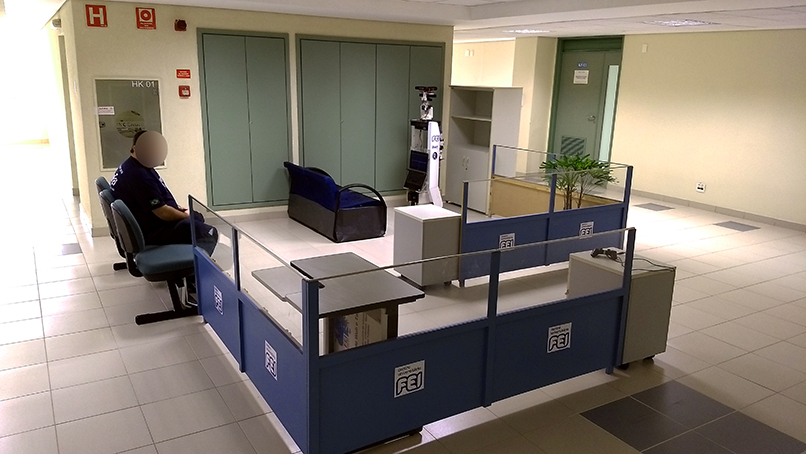
\includegraphics[width=\textwidth]{cenario.jpg}
		\smallcaption{Fonte: Autor.}
		\label{fig:cenario}
	\end{minipage}
\end{figure}

\subsection{Objetivo}

Verificar a compreensão e conforto da pessoa ao observar e interagir com o robô no ambiente doméstico, afim identificar experiências positivas e negativas por parte do usuário.

\subsection{Estados de Comportamento do Humano}

Para o teste são consideradas algumas possibilidades de posicionamento da pessoa e robô para interagirem:

\begin{itemize}
	\item Pessoa parada em pé e o robô inicia a interação próximo do usuário.
	\item Pessoa parada em pé e o robô inicia a interação distante do usuário.
	\item Pessoa parada sentada e o robô inicia a interação próximo do usuário.
	\item Pessoa parada sentada e o robô inicia a interação distante do usuário.
\end{itemize}

O objetivo das configurações é a aleatoriedade do posicionamento entre robô e pessoa, considerando cenários doméstico onde o convívio é comum. Assim, é possível medir a experiência do usuário em diversas situações de convivência.

\subsection{Tarefa do Robô}

Esse teste ocorre em um ambiente controlado, porém o trânsito de outros indivíduos pelo cenário acontece com frequência significativa. O passo a passo da tarefa é descrito na lista a seguir:

\begin{enumerate}
	\item \textbf{Início}: O robô é posicionado no cenário de maneira que esteja em um local em torno da residência simulada.
	\item \textbf{Busca pelo objeto}: O robô segue até uma mesa, ou armário, onde supostamente deixou sua garrafa.
	\item \textbf{Interação com a pessoa}: O robô se aproxima do usuário e questiona se ele viu a garrafa.
	\item \textbf{Nova busca pelo objeto}: O robô segue a um novo ponto em busca da garrafa, que novamente não está no local.
	\item \textbf{Retorno ao usuário}: O robô retorna ao local onde o usuário se encontra e, em uma distância maior ou menor de proximidade (aleatória), solicita que o usuário o acompanhe.
	\item \textbf{Fim}: Será considerado o fim da tarefa, quando o robô alcançar um ponto ao redor do cenário e informar o fim do teste ao participante.
\end{enumerate}

As tarefas são definidas com base no contexto de uso ilustrado através da figura~\ref{fig:contextouso}. Nesse ponto, o projeto está especificado, os equipamentos e ambiente prontos para realizar a interação humano-robô. Como é um experimento que envolve testes com ser humano, é importante enviar o projeto para apreciação do comitê de ética através da ferramenta Plataforma Brasil. Esse projeto tem a aprovação do comitê de ética, através do número de processo CAAE: 70057117.0.0000.5508, que pode ser lido na íntegra no apêndice~\ref{ap:projeto}.

\section{PREPARAÇÃO DO ROBÔ}
\label{sec:ec_robo}
O robô utilizado no desenvolvimento da tese é o PeopleBot~\footnote{PeopleBot - http://www.mobilerobots.com/researchRobots/PeopleBot.aspx} fabricado pela ActivMedia Robotics. Ele é um robô móvel com direção diferencial, ou seja, possui duas rodas motorizadas e uma roda castor que auxilia em seu equilíbrio. O projeto do PeopleBot tem foco em pesquisas e serviços que envolvem interação humano-robô. Com esse objetivo, ele foi desenvolvido com uma altura de 112 cm (centímetros). Além disso, o PeopleBot também possui uma garra pequena que tem sua movimentação apenas na direção vertical. A figura~\ref{fig:peoplebot} apresenta o robô PeopleBot.

\begin{figure}[ht!]
	\centering
	\begin{minipage}{\textwidth}
		\caption{Robô ActivMedia Robotics PeopleBot.}
		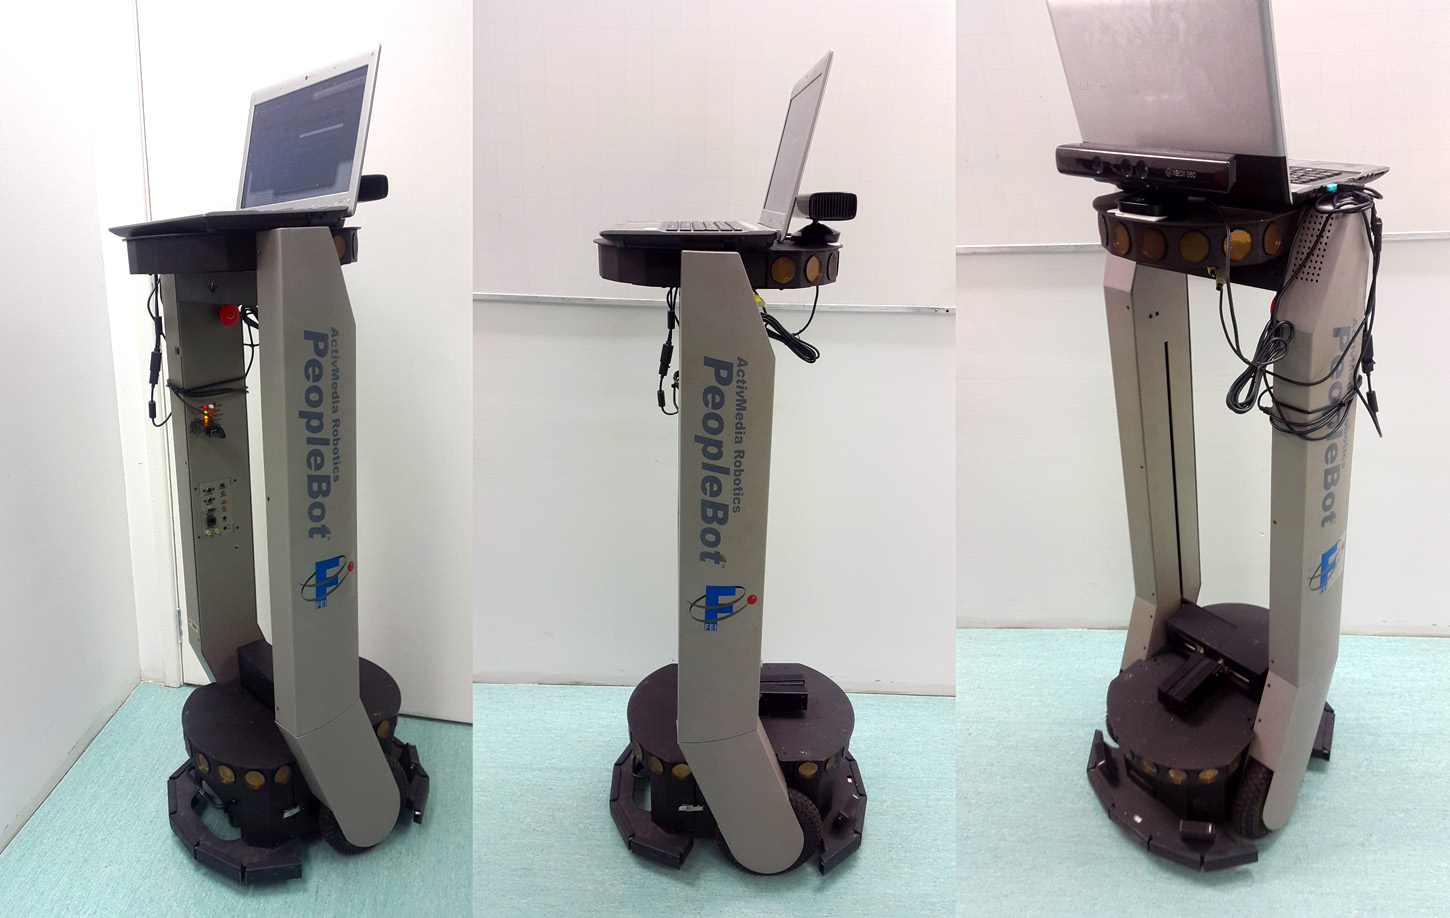
\includegraphics[width=\textwidth]{peoplebot.jpg}
		\smallcaption{Fonte: Autor.}
		\label{fig:peoplebot}
	\end{minipage}
\end{figure}

Como a garra do PeopleBot é curta e não permite muita destreza na manipulação de objetos e gestos, além de possuir poucos graus de liberdade, foi construído e adicionado um novo manipulador. O projeto do manipulador foi desenvolvido com o intuito de auxiliar a manipulação de objetos a uma certa distância e execução de gestos durante interações com pessoas. Esse novo manipulador é importante já que durante a interação social, seres humanos gesticulam para ilustrar a intenção e fala do que querem transmitir, por exemplo, acenar com as mãos ao falar olá. Esse tipo de comportamento aproxima naturalidade a interação humano-robô, podendo gerar um conforto a pessoa que interage. O projeto atende pesquisas com foco em prestação de serviços domésticos e cuidados pessoais, e foi construído de maneira que os movimentos sejam próximos do braço humano. O desenho que ilustra o manipulador desenvolvido é apresentado através da figura~\ref{fig:manipulador}. 

\begin{figure}[ht!]
	\centering
	\begin{minipage}{0.6\textwidth}
		\caption{Projeto do Novo Manipulador do PeopleBot.}
		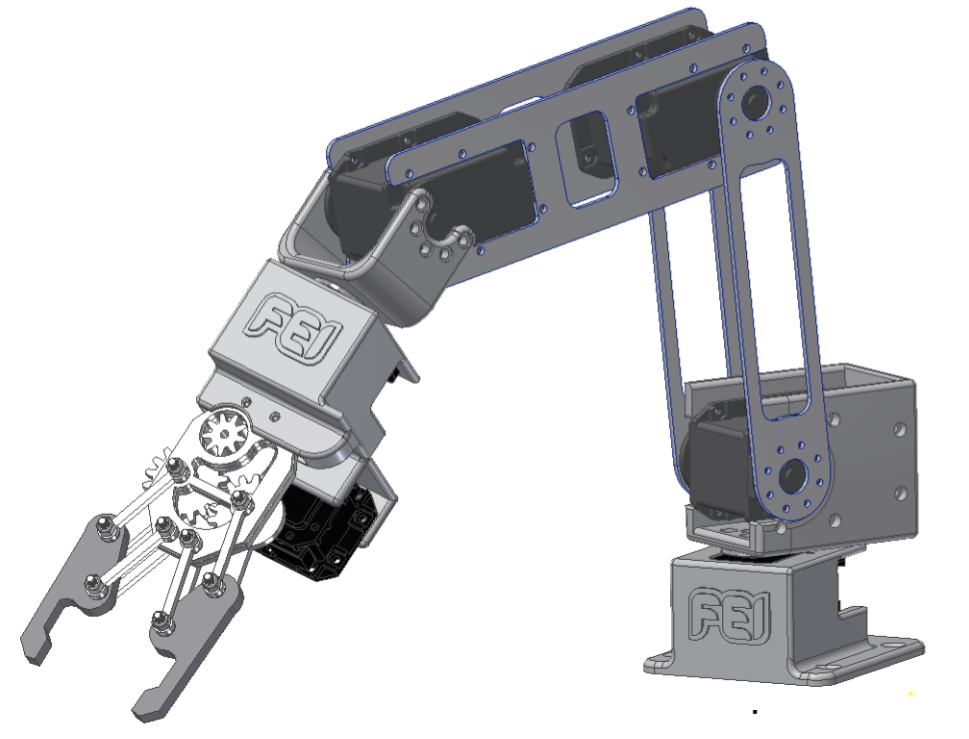
\includegraphics[width=\textwidth]{manipulador.png}
		\smallcaption{Fonte: \textcite{gonbata:2016}.}
		\label{fig:manipulador}
	\end{minipage}
\end{figure}

Além do manipulador, também foi acoplado um \emph{tablet} para que seja possível atribuir face ao robô e consequentemente expressões faciais, deixando a interação mais amigável. O projeto da cabeça do robô é apresentado na figura~\ref{fig:judithhead}.

\begin{figure}[ht!]
	\centering
	\begin{minipage}{0.4\textwidth}
		\caption{Projeto da Cabeça para o PeopleBot.}
		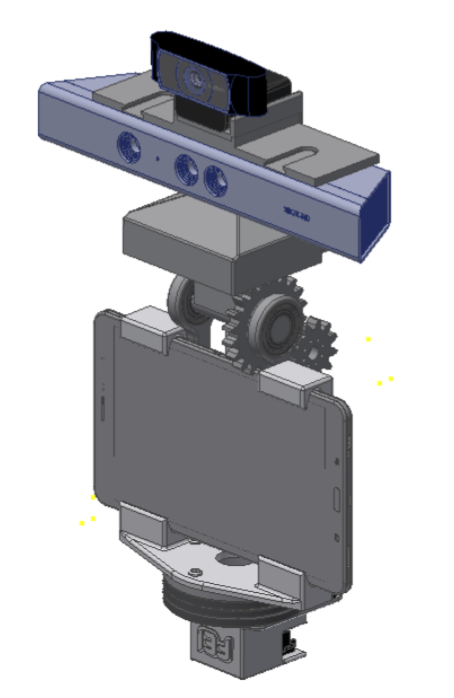
\includegraphics[width=\textwidth]{judith_head.png}
		\smallcaption{Fonte: \textcite{gonbata:2016}.}
		\label{fig:judithhead}
	\end{minipage}
\end{figure}

O projeto da cabeça foi preparado para acoplar alguns sensores como o Microsoft\textregistered\ Kinect\textregistered\ , o ASUS\textregistered\ Xtion\textregistered\ e webcams, para tarefas que envolvam nuvem de pontos de profundidade e visão computacional. Sensores como \emph{laser}s e microfones também foram instalados para melhorar a captura de informações sobre o ambiente e interagir melhor com a pessoa. O sensor \emph{laser} utilizado foi o Hokuyo URG-04LX-UG01 que possui um alcance de 5 metros, suficiente para navegação em um ambiente doméstico. O microfone, por se tratar de um ambiente com ruído e que a interação possuí diferentes distâncias para ocorrer, optou-se por um tipo \emph{shotgun} que tem o alcance de aproximadamente 2 metros. O modelo do microfone é o RODE Videomic Pro. O desenvolvimento do manipulador e da cabeça do robô foram realizados no projeto apresentado por \textcite{gonbata:2016} que ocorreu em paralelo, durante a preparação do robô.

Durante os primeiros testes, a base do Peoplebot sofreu uma avaria e foi substituída por uma base da KUKA. É uma base com rodas omnidirecionais que proporcionam uma maior mobilidade de direções para o robô. A figura~\ref{fig:newjudith} apresenta a montagem final do robô para realização dos testes de interação na residência.

\begin{figure}[ht!]
	\centering
	\begin{minipage}{0.4\textwidth}
		\caption{Robô Judith na sua montagem final.}
		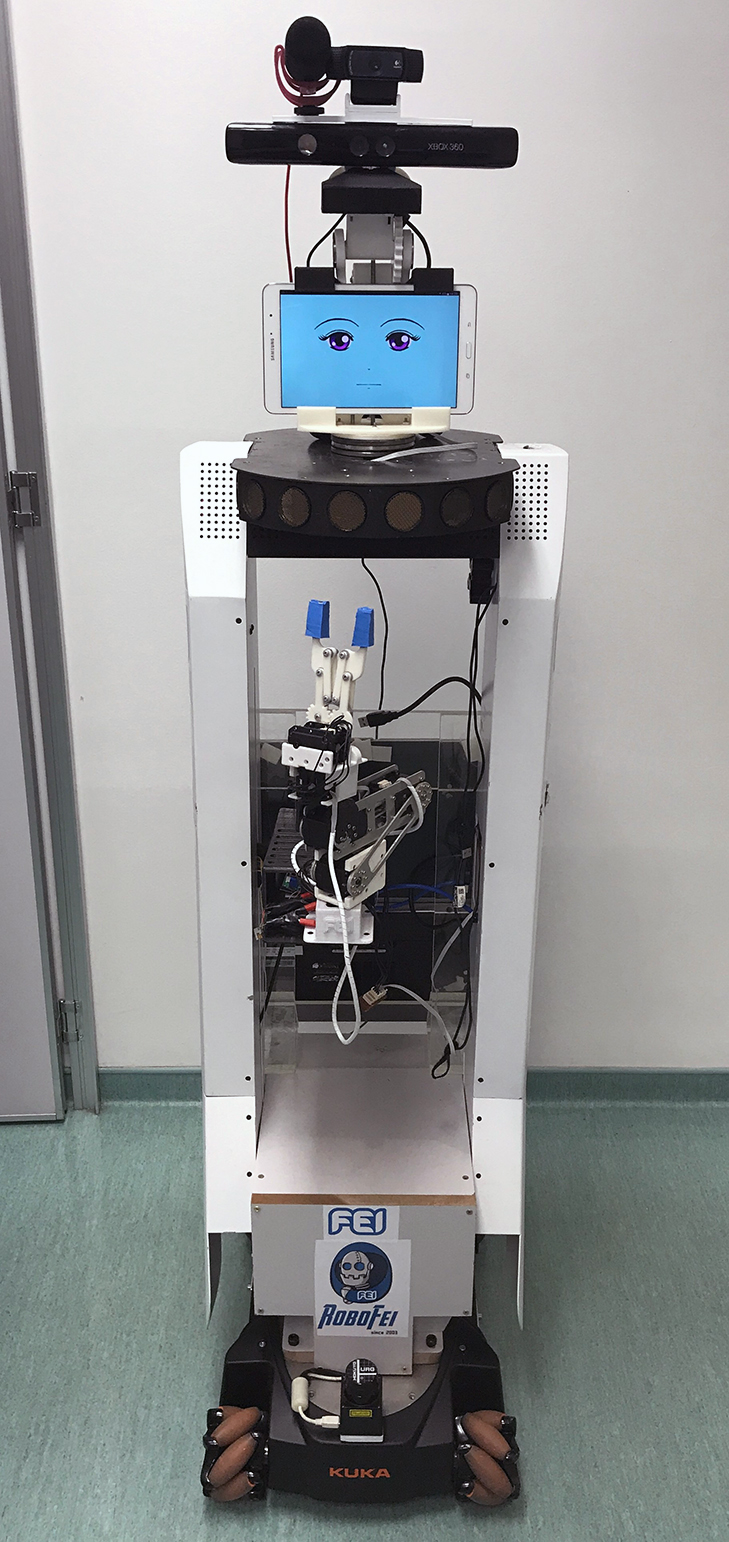
\includegraphics[width=\textwidth]{judith.jpg}
		\smallcaption{Fonte: Autor.}
		\label{fig:newjudith}
	\end{minipage}
\end{figure}

Além dos preparativos mecânicos para possibilitar a execução, de cada comportamento que atende as funcionalidades do projeto, também é necessário preparar os \emph{softwares} que irão compor a inteligência do robô. A arquitetura do robô e bibliotecas utilizadas para a composição do \emph{software} são apresentadas nas seções a seguir.

\subsection{Arquitetura do Software} %ATUALIZAR COM O TEXTO DO CADERNO
\label{sec:arquitetura}
A arquitetura construída para o software do robô foi feita em camadas. Ela segue as diretrizes de arquitetura do ROS. O nó \textit{master}, criado ao inicializar o ROS, cria um servidor DNS. A partir desse servidor, novos nós são conectados através de um protocolo TCP/IP utilizando biblioteca de \textit{socket}. Após conectado, um nó, pode enviar uma mensagem de comunicação via protocolo de rede. Essa mensagem é distribuída através do processo de \textit{broadcast}. Isso significa que o nó fica emitindo informações na rede, sem um alvo específico e qualquer indivíduo dentro da rede pode interceptar essas informações. As mensagens são publicadas através de tópicos. A partir desse ponto, qualquer nó que queira ler a mensagem pode se inscrever no tópico. A ilustração dessa operação é apresentada através de figura~\ref{fig:ros_works}.

\begin{figure}[ht!]
	\centering
	\begin{minipage}{0.6\textwidth}
		\caption{Ilustração do funcionamento do ROS.}
		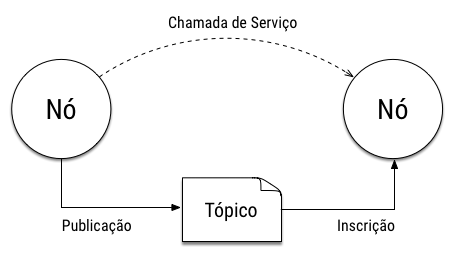
\includegraphics[width=\textwidth]{ros_works.png}
		\smallcaption{Fonte: Autor.}
		\label{fig:ros_works}
	\end{minipage}
\end{figure}

Dessa forma é fácil separar os códigos responsáveis em pacotes e camadas que mantenham um funcionamento independente. Então quando for necessário adicionar um novo código ou funcionalidade, basta criar um novo pacote ou um novo nó que irá atendê-la. Assim, o pacote approach\_control foi desenvolvido. A figura~\ref{fig:arquitetura} apresenta as camadas do pacote approach\_control construído com base nos princípios do ROS.

\begin{figure}[ht!]
	\centering
	\begin{minipage}{0.9\textwidth}
		\caption{Arquitetura do projeto para o classificador Bayesiano.}
		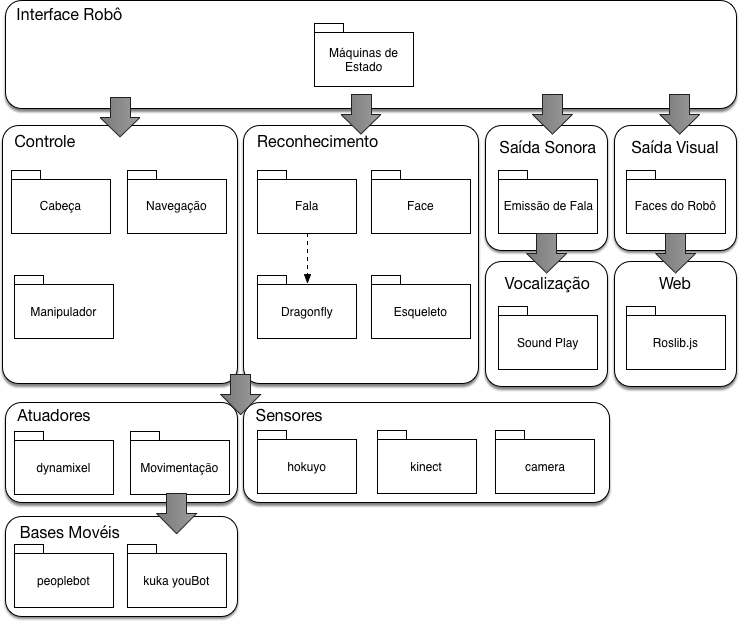
\includegraphics[width=\textwidth]{arquitetura.png}
		\smallcaption{Fonte: Autor.}
		\label{fig:arquitetura}
	\end{minipage}
\end{figure}

As camadas forma divididas em 9 principais grupos. Cada grupo tem um objetivo específico. A primeira é a interface do robô, que através das máquinas de estado, controlam a comunicação entre todos os nós do sistema e o robô. A camada de controle concentra todos os pacotes que fazem os algoritmos de controle e determinam os parâmetros dos atuadores do robô. A camada de reconhecimento possui todos os algoritmos de reconhecimento utilizados no robô. Nela estão os pacotes para reconhecimento de face e gênero, que utilizam o \textit{framework} OpenCV, do esqueleto do usuário, através da biblioteca do PyOpenNI e o de fala que redireciona o que foi recebido para o DragonFly, que implicitamente utiliza o Windows Speech para reconhecer a fala. Saída sonora é uma camada que trata apenas o evento para uma chamada ao programa de reprodução de áudio SoundPlay, que é nativo ao sistema operacional Linux. Ele ficou em uma camada separada, pois pode inserir qualquer outro programa de reprodução de voz. Em uma camada separada, facilita a expansão e mudança de \textit{softwares} utilizados e também o uso de outros pacotes.

A camada de saída visual tem uma página HTML que utiliza uma outra camada web para deixar a face do robô dinâmica. Ela trabalha com as mensagens enviadas na rede do ROS e recebe essas informações através do componente roslib.js que é um \textit{wrapper} para a camada interna TCP/IP criada através do nó master. Também foi criado uma camada de atuadores e sensores que mantém a última versão funcional dos pacotes que possuem os \textit{drivers} de comunicação de cada uma das bases robóticas utilizadas no projeto do estudo de caso do método centrado no usuário de interação humano-robô. A relação entre os pacotes criados e existentes no repositório approach\_control~\footnote{https://github.com/amasiero/approach\_control} pode ser observado através da figura~\ref{fig:pacotes}.

\begin{figure}[ht!]
	\centering
	\begin{minipage}{0.9\textwidth}
		\caption{Arquitetura de componentes que representam os softwares construídos no pacote approach\_control.}
		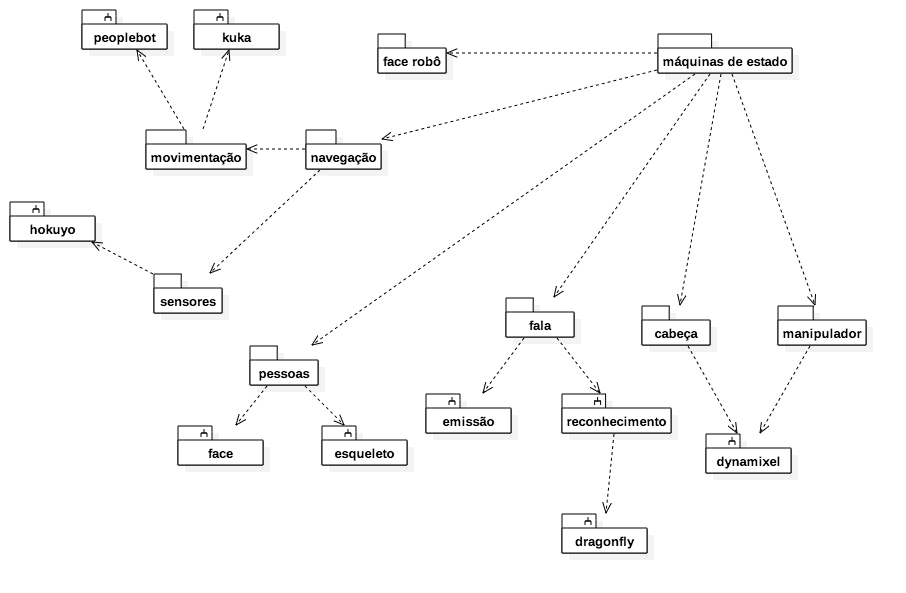
\includegraphics[width=\textwidth]{pacotes.png}
		\smallcaption{Fonte: Autor.}
		\label{fig:pacotes}
	\end{minipage}
\end{figure}

Essa estrutura permite a expansão e também a troca de algoritmos, \textit{softwares} e componentes de maneira mais fácil e sem muito esforço ou retrabalho ao codificar as novas soluções, além da refatoração do código fonte do robô ser mínima.


\subsection{Bibliotecas}
\label{sec:bibliotecas}
Para auxiliar no desenvolvimento da tese, algumas bibliotecas e softwares foram utilizados. O primeiro, conforme dito na seção~\ref{sec:arquitetura}, foi o ROS que é um \emph{framework} para desenvolvimento de software em robôs. Ele roda sobre o Ubuntu Linux, que no caso da tese foi utilizado a versão 14.04, com o ROS versão Indigo.

A biblioteca que gerencia a máquina de estados criada para execução das tarefas é o SMACH~\footnote{http://wiki.ros.org/smach}. Ele possibilita a criação e realiza o gerenciamento dos estados durante a execução das ações do robô. Para reconhecimento de voz a biblioteca utilizada foi o Dragonfly Speech Recognition~\footnote{https://pypi.python.org/pypi/dragonfly/0.6.5}. Bibliotecas como o OpenCV~\footnote{http://opencv.org/}, PyOpenni~\footnote{https://github.com/jmendeth/PyOpenNI} e MoveIt!~\footnote{http://moveit.ros.org/} foram utilizados para percepção e interação com o ambiente e também com o usuário. O programa que realiza a interação da face do robô foi desenvolvido em HTML e Javascript. Ele encontra-se disponível através do endereço \url{https://github.com/amasiero/robot\_face}.

Todos os pacotes desenvolvidos utilizaram a linguagem de programação Python, que possibilitou diversas facilidades na implementação dos códigos e integração das camadas dos pacotes no ROS. Para criação e teste da rede Bayesiana proposta utilizou-se o \emph{framework} SamIam~\footnote{http://reasoning.cs.ucla.edu/samiam/}, que realiza os cálculos de todas as probabilidades de uma consulta a rede de maneira objetiva.


\section{TESTES PILOTO}
\label{sec:ec_testespiloto}
Antes de realizar o teste piloto é importante que o projeto submetido ao comitê de ética esteja aprovado, vide apêndice~\ref{ap:projeto}. Nesse ponto o usuário é convidado a interagir com o robô. O especialista posiciona o usuário no ambiente de teste, onde ele pode ficar sentado ou em pé. Câmeras são posicionada de maneira que o possam capturar as reações que o usuário terá durante toda a interação com o robô. O especialista explica todos os procedimentos do experimento e da o sinal para que o robô inicie o teste. O sinal ocorre através de um comando de voz para o robô. Durante todo o experimento o usuário é incentivado a falar em voz alta o que está passando pela sua cabeça. Com as informações faladas e observações visuais, que são feitas pelo próprio especialista, são gerados pontos de atenção para melhoria e até pontos de sucesso no projeto. Ao final, o usuário é encaminhado para preencher o questionário pós teste, apresentado em detalhes na seção~\ref{sec:questionarioposteste}.

É importante delimitar os usuários que farão os testes de maneira criteriosa. Os perfis dos selecionados podem levar a diferentes resultados na interação. Os usuários selecionados para realizar o teste, são denominados de sujeito de teste. Nessa tese o seguinte perfil foi utilizado: pessoas que possuem idades diversificadas com variedade de 18 a 70 anos. Alguns candidatos ao teste possuem medo declarado de robôs e neste caso o especialista ficará acompanhando o teste com uma maior proximidade para evitar problemas com o robô e principalmente com a pessoa.

São evitados a repetição de configuração entre os candidatos, para que não seja levantado nenhum conhecimento a priori sobre o comportamento do robô.

\subsection{Heurísticas de Interação Humano-Robô}
\label{sec:heuristicas}
Durante os testes piloto, percebeu-se que algumas heurísticas de avaliação de interação foram percebidas pelo usuário. Dessa maneira, foi realizado um trabalho para inclusão das variáveis na lista de variáveis de observação. 

Avaliação heurística é um método utilizado por especialistas em usabilidade para verificar problemas de interação em interfaces de sistemas e produtos. \citeonline{nielsen:1994} apresenta 10 heurísticas para avaliações de interfaces em sistemas web (vide seção~\ref{sec:avaliacao}). As heurísticas de Nielsen têm sido amplamente utilizadas ao longo dos tempos para sites e sistemas desktop. Alguns trabalhos discutidos ao longo da seção~\ref{sec:ihrux} apresentam modificações das heurísticas de Nielsen para o cenário de interação humano-robô.

Nos questionários pré e pós teste preenchido pelos usuários, notou-se que apontavam no robô a falta ou a presença de características que representavam as heurísticas de avaliação. Cada usuário dava mais atenção a determinadas características, que compunham diferentes perfis de interação. Assim, as heurísticas de avaliação apresentadas pela literatura foram estudadas. A partir desse estudo, verificou-se que as heurísticas mais presentes nos comentários dos usuários, também estavam presentes nas listas contidas na literatura. Dentre as heurísticas que apresentam uma descrição de maior aplicabilidade em robótica social e interação humano-robô estão as heurísticas de \citeonline{clarkson:2007} (vide tabela~\ref{tab:heuristicasihr}).

Nesse momento é realizado a seleção das heurísticas em comum com os comentários dos usuários. Essas heurísticas são transformadas em variáveis que compõem a rede bayesiana, a fim de auxiliar na classificação do perfil do usuário em interação. Com base nas observações e comentários dos testes de interação, mais os estudos da literatura, foi possível identificar as seguintes heurísticas para transformá-las em variáveis que formam o conjunto de classificação do usuário:

\begin{itemize}
	\item Visibilidade do estado do sistema;
	\item Uso de sugestões naturais;
	\item Síntese do sistema e interface;
	\item Ajudar o usuário a reconhecer, diagnosticar, e recuperar de erros.
\end{itemize}

Cada uma das heurísticas apresentadas na lista acima, foram observadas durante os testes através dos comentários dos participantes. Assim, elas apresentam dependência condicional com os perfis e/ou com as ações do robô. Por exemplo, sobre a questão da visibilidade do estado do sistema (robô), alguns participantes comentaram que o robô poderia sempre informar os próximos passos. Esse comportamento faria com que o participante ficasse mais confortável com o robô pela casa. Sobre a questão da naturalidade dos movimentos e fala, participantes não conseguiram entender os gestos do manipulador, até o que robô falasse algo que complementa os gestos. Isso ocorreu também devido às limitações físicas do manipulador desenvolvido (vide figura~\ref{fig:manipulador}). Após avaliar as heurísticas de \textcite{clarkson:2007} com os comentários dos usuários, definiu-se o conjunto de heurísticas apresentado acima.

\section{CRIAÇÃO DAS PERSONAS}
\label{sec:ec_personas}
A execução do QG-SIM foi realizada com três valores Q diferentes, 0.6, 0.7 e 0.8. Após cada execução é verificado como foi realizado o agrupamento, para que não existam grupos muito generalizados e nem grupos muito especializados. Para o valor $Q = 0.6$, foram encontrados 3 grupos, dois grupos com 1 pessoa cada e um grupo contendo os demais perfis. Ficou muito generalizado. O próximo valor testado foi de $Q = 0.8$. Nesse caso, o resultado foi muito específico, pois houve 9 grupos sendo grande parte com 1 ou 2 perfis e poucos grupos com 5 perfis. O valor intermediário $Q = 0.7$, apresentou um comportamento melhor onde encontrou 5 grupos. 2 grupos com 1 perfil cada, 1 grupo com 7, outro com 9 e o maior com 21. Alguns fatores, como idade, redes sociais, contato com robôs, entre outros foram determinantes para esse resultado. Detalhes sobre cada grupo é apresentado no capítulo~\ref{cap:resultados}. Agora que os grupos estão definidos, deve-se criar as Personas que representam cada um deles. 

Cinco Personas foram construídas. Essas são apresentadas nas tabelas~\ref{tab:joaquim}, \ref{tab:mariaeduarda}, \ref{tab:alfredo}, \ref{tab:danielo} e \ref{tab:manuel}, a seguir.

\begin{table}[!ht]
	\caption{Persona Joaquim}
	\label{tab:joaquim}
	\centering
	\begin{tabular}{ m{2 cm} | m{13cm} }
		\hline
		Foto: & \rule{0cm}{2.7cm} 
\includegraphics[scale=0.8]{joaquim.png} \\
		\hline
		Nome: & Joaquim \\
		\hline
		Descrição: & Tem 21 anos, 1,71 m de altura, em geral não é uma pessoa séria ou carrancuda, mas também não é sorridente. É um homem \textbf{sociável}, cheio de amigos a sua volta e adora ir ao barzinho com eles. Mora na capital paulista, centro econômico brasileiro, local perfeito para um homem que gosta de variedade cultural. \textbf{Não fica longe de seu smartphone e também sempre que pode, está com seu laptop no colo navegando pelo Facebook e postando fotos no Instagram}. Tudo que pode ser resolvido pelo seu smartphone ele faz, seja por chamada de voz ou qualquer aplicativo. Mas, ainda não conseguiu se habituar aos serviços financeiros digitais, prefere o método clássico para guardar seu dinheiro, o colchão. Nunca viajou para fora do Brasil, inclusive seu mapa de viagens nacionais também não é extenso. Ao todo, visitou apenas 9 cidades do Brasil com o passar do tempo.

		Na universidade acompanhou os times de robótica nas competições e teve contato com diversos tipos de robôs, como os parecidos com humanos e animais, com mobilidade através de rodas e também os de linha de produção. Quando perguntam sua expectativa sobre robôs convivendo em sua casa, ele diz que tudo bem, desde que ele execute as \textbf{tarefas domésticas sempre com obediência e de certa maneira, também espera que o robô seja afetivo na interação}. Um comportamento próximo ao de uma diarista na família. Já no ambiente industrial, Joaquim acredita que os robôs são apenas ferramentas de trabalho e não devem fazer nada além de executar o que lhe foi programado. \\
		\hline
	\end{tabular}
	\smallcaption{Fonte: O autor.}
\end{table}

\begin{table}[!ht]
	\caption{Persona Maria Eduarda}
	\label{tab:mariaeduarda}
	\centering
	\begin{tabular}{ m{2 cm} | m{13cm} }
		\hline
		Foto: & \rule{0cm}{2.7cm} 
\includegraphics[scale=0.8]{maria_eduarda.png} \\
		\hline
		Nome: & Maria Eduarda \\
		\hline
		Descrição: & Aos 36 anos, com 1,71 m de altura, é uma garota reservada que adora sorrir em diversas ocasiões. É \textbf{bem sociável, e mantém os amigos por perto}. É uma mulher moderna e gosta de manter seu corte de cabelo mais curto que o convencional. Mora em São Bernardo do Campo, cidade da grande São Paulo e gosta muito de visitar o interior de São Paulo para passar seus feriados prolongados. Não vive sem seu celular, e no trabalho o computador é sua principal ferramenta. Quando está em \textbf{casa utiliza sua Smart TV para assistir suas séries e filmes favoritos}. Gostaria muito de ter um leitor de e-book para evitar carregar livros pesados durante seu trajeto pelo transporte público. Mesmo com essa adoção a tecnologia, empresas digitais, principalmente do mercado financeiro, não a atraem. Sempre \textbf{conectada através do celular, ela posta tudo no Facebook, tanto de trabalho quanto de lazer}.

		Já viajou algumas vezes para os EUA, sempre a passeio com o principal destino a Disney. Pelo Brasil, já viajou para algumas cidades fora de São Paulo e deixou sua marca por todas as regiões do país. Como ela trabalha em uma universidade de engenharia, já viu diversos tipos de robôs, que são utilizados nas aulas. Porém, nunca teve um contato direto com eles, a não ser seu aspirador de pó. Tanto em casa quanto no trabalho, ela espera que \textbf{robôs sejam capazes de realizar tarefas com eficácia, como dirigir um carro, digitar planilhas, mas que ao mesmo tempo não seja capaz de substituí-la}.\\
		\hline
	\end{tabular}
	\smallcaption{Fonte: O autor.}
\end{table}

\begin{table}[!ht]
	\caption{Persona Alfredo}
	\label{tab:alfredo}
	\centering
	\begin{tabular}{ m{2 cm} | m{13cm} }
		\hline
		Foto: & \rule{0cm}{2.7cm} 
\includegraphics[scale=0.8]{alfredo.png} \\
		\hline
		Nome: & Alfredo \\
		\hline
		Descrição: & Aos 24 anos, rapaz de estatura normal, por volta de 1,75m, está sempre com um belo sorriso no rosto, faça chuva ou faça sol. Sempre \textbf{tem pessoas a sua volta, gosta de contar piadas e fazer todos sorrirem}. Morador da cidade de São Bernardo do Campo, mas sempre que pode vai para o litoral paulista visitar os pais e curtir uma praia. Usa computador para fazer os trabalhos da faculdade e \textbf{passa grande parte do seu tempo no celular}. Não possui serviços financeiros digitas, pois ainda não conseguiu a aprovação do cadastro. Quando se trata de internet banking, \textbf{acredita que o seu computador é mais seguro que o uso de celular}.

		Alfredo vive antenado nas redes sociais, como Twitter, Instagram e Facebook. Ajudam ele a ficar conectado com as últimas notícias e eventos a sua volta. Tem um sonho de viajar para o exterior, mas isso ainda não foi possível, em compensação pelo Brasil já visitou mais de 30 cidades, a maioria na região Sudeste. Na universidade, através do curso de engenharia de automação, teve contato com robôs de fábrica e móveis conforme os laboratórios das disciplinas ocorriam. Quando perguntam a Alfredo o que ele espera de um robô doméstico e também um robô no trabalho, ele diz que \textbf{robôs devem executar as tarefas propostas de maneira eficiente e que sua interação seja toda por comando de voz}.\\
		\hline
	\end{tabular}
	\smallcaption{Fonte: O autor.}
\end{table}

\begin{table}[!ht]
	\caption{Persona Danielo}
	\label{tab:danielo}
	\centering
	\begin{tabular}{ m{2 cm} | m{13cm} }
		\hline
		Foto: & \rule{0cm}{2.7cm} 
\includegraphics[scale=0.8]{danielo.png} \\
		\hline
		Nome: & Danielo \\
		\hline
		Descrição: & Com 27 anos de idade, 1,83m, Danielo está sempre na \textbf{academia para treinar com seus amigos}. Mora em São Bernardo do Campo, e utiliza seu computador para fazer seu trabalho e o celular para manter contato com seus amigos. \textbf{Nunca quis saber de leitores de e-book, pois acha sua tecnologia sem utilidade nos dias atuais}. A sua única rede social é o Facebook. Ele acha que já toma tempo o suficiente e não precisa de outras para ver a mesma coisa. Danielo é um rapaz que já viajou bastante. Já visitou 3 países latinos e no Brasil visitou mais de 90 cidades, concentradas em sua grande parte, na região Sudeste. O contato com robôs é limitado e restrito a robôs de fábrica. Em casa \textbf{ele acredita que o robô será parecido com seres humanos para fazer as atividades domésticas, e no trabalho substituirão seres humanos em trabalhos repetitivos}, como nas fábricas e linha de produção.\\
		\hline
	\end{tabular}
	\smallcaption{Fonte: O autor.}
\end{table}

\begin{table}[!ht]
	\caption{Persona Manuel}
	\label{tab:manuel}
	\centering
	\begin{tabular}{ m{2 cm} | m{13cm} }
		\hline
		Foto: & \rule{0cm}{2.7cm} 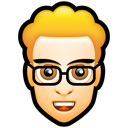
\includegraphics[scale=0.8]{manuel.png} \\
		\hline
		Nome: & Manuel \\
		\hline
		Descrição: & Aos 33 anos, 1,85 m,  Manuel um professor universitário sempre sorridente. Seus alunos sempre o procuram para esclarecer dúvidas e pedir conselhos. Mora em São Bernardo do Campo, próximo ao seu local de trabalho, por que adora o conforto de ir em sua casa poder almoçar uma comida fresca. Acredita que tem uma melhor qualidade de vida assim. \textbf{Não é muito fã de tecnologia de ponta, então fica contente em ter seu computador, onde resolve tudo que pode. Digitalmente, considera-se antissocial e não mantém cadastro em nenhuma rede social}.

		Já visitou países pela Europa, África, América do Norte e do Sul. No Brasil, seu foco de visitar está na região Sudeste, principalmente o estado de Minas Gerais. No total já percorreu mais de 62 cidades pelo país. Como professor, sua linha de pesquisa principal de estudos é a robótica, fazendo com que tenha contato com todos os tipos de robôs. \textbf{Em casa, pensa em ter um robô para atender suas necessidades}, assim como no trabalho. Porém, o robô \textbf{no trabalho deve atender também as necessidades e expectativas da empresa}.\\
		\hline
	\end{tabular}
	\smallcaption{Fonte: O autor.}
\end{table}

As Personas apresentadas nas tabelas~\ref{tab:joaquim}, \ref{tab:mariaeduarda}, \ref{tab:alfredo}, \ref{tab:danielo}, \ref{tab:manuel} ajudaram na definição das independências condicionais entre as variáveis da rede bayesiana. Mais informações das análises feitas com base nas Personas, e também sobre sua criação, em relação a interação com o robô são apresentadas no capítulo~\ref{cap:resultados}.

\section{TOMADA DE DECISÃO: CLASSIFICADOR BAYESIANO}
\label{sec:rede-bayesiana}
Neste momento todos os passos necessários para identificar as Personas, ações do robô e as necessidades do projeto foram realizados. As últimas variáveis selecionadas para compor a rede Bayesiana para classificação do perfil do usuário, representado pela Persona, são as comportamentais. As variáveis comportamentais neste ponto estão ligadas as possíveis experiências que o usuário pode sentir na interação. Dentre as variáveis apresentadas na seção~\ref{sec:ec_variaveis} são selecionadas as variáveis conforto e medo. As duas variáveis conseguem representar grande parte das demais variáveis comportamentais. Neste momento, a forma de identificar as variáveis de conforto e medo, é através da declaração do usuário durante o teste e também nas respostas do questionário pós teste. A partir desse ponto, têm-se todas as variáveis definidas e é necessário definir a estrutura da rede Bayesiana. Na sequência será apresentado cada conjunto de nós e suas dependências condicionais para a criação da estrutura da rede Bayesiana de classificação, dado as especificações do projeto de interação humano-robô, de acordo com o método apresentado no capítulo~\ref{cap:projetoihr}.

Os nós raízes da rede Bayesiana são compostos pelas 5 Personas apresentadas na seção~\ref{sec:ec_personas}. Elas são escolhidas como raiz por que representam os perfis de usuários que devem ser classificados durante a aproximação do robô. A probabilidade do usuário em interação ser ou não aquela Persona é determinada, pela quantidade de pessoas que pertencem ao grupo encontrado pelo QG-SIM. Como são nós raízes, não existem nenhuma evidência para compor seu valor de probabilidade, apenas a quantidade de pessoas de cada grupo. As equações~\ref{eq:joaquim}, \ref{eq:mariaeduarda}, \ref{eq:alfredo}, \ref{eq:danielo} e \ref{eq:manuel} representam a probabilidade de cada uma das Personas obtidas.

\begin{equation}
	\label{eq:joaquim}
	P(joaquim)
\end{equation}

\begin{equation}
	\label{eq:mariaeduarda}
	P(maria\_eduarda)
\end{equation}

\begin{equation}
	\label{eq:alfredo}
	P(alfredo)
\end{equation}

\begin{equation}
	\label{eq:danielo}
	P(danielo)
\end{equation}

\begin{equation}
	\label{eq:manuel}
	P(manuel)
\end{equation}

As variáveis são nomeadas com letras minúsculas, pois são variáveis com apenas dois valores representando ser ou não ser. Essa notação segue a convenção apresentada por \citeonline{russell:2002}.

Seguindo com a construção da rede, cada nó interno foi considerado com base nas variáveis criadas a partir das heurísticas de interação humano-robô, das ações do robô e também do contexto de uso e ambiente de teste. As independências condicionais entre cada nó foram observadas pelos comentários de cada usuário durante os testes. O processo de criação dos nós é detalhado na sequência. A inclusão dos nós é feita com base nas variáveis apresentadas na tabela~\ref{tab:variaveisvalores}.

O nó Proximidade leva em consideração os espaços sociais definidos por \citeonline{hall:1969}. O domínio foi simplificado para \{perto, longe\}, pois durante os testes pilotos a reação do usuário era a mesma entre as regiões íntima e pessoal (perto) e as regiões social e pública (longe). A dependência condicional foi aplicada de acordo com a declaração explícita entre os perfis que sentiram algum desconforto com a aproximação do robô. A equação~\ref{eq:proximidade} define o cálculo de probabilidade condicional para a variável aleatória Proximidade.

\begin{equation}
	\label{eq:proximidade}
	P(proximidade | joaquim, alfredo, danielo)
\end{equation}

A próxima variável aleatória inserida é a Posição da pessoa no ambiente. O domínio dessa variável é determinado por \{sentado, em pé\}. Ela foi observada durante a prova de reconhecimento de pessoas e aproximação do robô na RoboCup de 2016. Nesse cenário, as pessoas que estavam sentadas ficavam bem desconfortáveis com a aproximação do robô, principalmente com relação ao seu manipulador. Nos testes pilotos, a situação demonstrou-se a mesma. As pessoas que estavam sentadas demonstravam um comportamento mais apreensivo do que as em pé. A equação~\ref{eq:posicao} apresenta o cálculo de probabilidade condicional para a variável Posicao.

\begin{equation}
	\label{eq:posicao}
	P(posicao | joaquim, maria\_eduarda, alfredo, danielo, manuel)
\end{equation}

As 4 próximas variáveis aleatórias descritas são referentes a ações do robô. Todos os 4 conjuntos são importantes na interação social e geram diferentes reações aos perfis de usuários. Um ponto interessante a ser ressaltado é que cada Persona mapeada, ficou atenta durante a interação em apenas algumas das variáveis. As 4 variáveis são Expressão Facial (equação~\ref{eq:face}), Gestos (equação~\ref{eq:gestos}), Estilo da Fala (equação~\ref{eq:fala}) e Velocidade (equação~\ref{eq:velocidade}). Seus respectivos domínios estão descritos na tabela~\ref{tab:variaveisvalores}.

\begin{equation}
	\label{eq:face}
	P(face | joaquim, maria\_eduarda, alfredo, danielo, manuel)
\end{equation}

\begin{equation}
	\label{eq:gestos}
	P(gestos | maria\_eduarda, alfredo, danielo, manuel)
\end{equation}

\begin{equation}
	\label{eq:fala}
	P(fala | joaquim, alfredo, danielo, manuel)
\end{equation}

\begin{equation}
	\label{eq:velocidade}
	P(velocidade | joaquim, maria\_eduarda)
\end{equation}

A partir da variável Gestos, observou-se que quando ocorreu o toque do robô na pessoa, gerou uma situação de medo. A variável toque é mapeada com a dependência condicional da variável Gestos (equação~\ref{eq:toque}). Seu domínio é binário, $\{toque, \neg toque\}$.

\begin{equation}
	\label{eq:toque}
	P(toque | gestos)
\end{equation}

Cada heurística apontada na seção~\ref{sec:heuristicas} gerou um nó que representa uma variável aleatória da rede Bayesiana. Todas as heurísticas utilizadas, possuem relação com os comportamentos do robô durante os testes de interação e também com as informações feitas pelos usuários. A lista a seguir mostra as heurísticas e as nomeações como variáveis aleatórias da rede Bayesiana.

\begin{itemize}
	\item Visibilidade do estado do sistema - estado\_robo (equação~\ref{eq:estadorobo});
	\item Uso de sugestões naturais - natural (equação~\ref{eq:natural});
	\item Síntese do sistema e interface - síntese (equação~\ref{eq:sintese});
	\item Ajudar o usuário a reconhecer, diagnosticar, e recuperar de erros - ajudar (equação~\ref{eq:ajudar}).
\end{itemize}

\begin{equation}
	\label{eq:estadorobo}
	P(estado\_robo | joaquim, alfredo, manuel)
\end{equation}

\begin{equation}
	\label{eq:natural}
	P(natural | fala, gestos)
\end{equation}

\begin{equation}
	\label{eq:sintese}
	P(sintese | fala)
\end{equation}

\begin{equation}
	\label{eq:ajudar}
	P(ajudar | maria\_eduarda, alfredo)
\end{equation}

Por fim, são definidas as variáveis aleatórias chamadas de nós evidências da rede Bayesiana. Esses nós correspondem ao sentimento das pessoas durante a interação com o robô. Esses sentimentos são declarados pelas pessoas durante a interação de acordo com o comportamento do robô. A composição das relações com esses nós foi dada pela observação dos testes e também das declarações realizadas através do questionário pós interação. As três variáveis aleatórias são conforto~\ref{eq:conforto}, desconforto~\ref{eq:desconforto} e medo~\ref{eq:medo}.

\begin{equation}
	\label{eq:conforto}
	P(conforto | proximidade, face, estado\_robo, natural, sintese)
\end{equation}

\begin{equation}
	\label{eq:desconforto}
	P(desconforto | posicao, face, estado\_robo, ajudar, natural)
\end{equation}

\begin{equation}
	\label{eq:medo}
	P(medo | velocidade, face, toque)
\end{equation}

As variáveis conforto e desconforto estão separadas, pois em alguns casos existiram pequenas diferenças que em uma mesma ação do robô, alguns usuários sentiram conforto e desconforto ao mesmo tempo. Por exemplo, ao se aproximar o robô chegou muito perto o que gerou o desconforto já que o usuário estava sentado, mas a expressão facial apresentada pelo robô no momento deixou ele tranquilo e confortável, mesmo não tendo como escapar da frente do robô (vide capítulo~\ref{cap:resultados}).

A figura~\ref{fig:rb} apresenta a estrutura completa da rede Bayesiana criada ao longo dessa seção.

\begin{figure}[ht!]
	\centering
	\begin{minipage}{\textwidth}
		\caption{Rede bayesiana construída para auxiliar no diagnóstico e avaliação da experiência do usuário na interação com o robô.}
		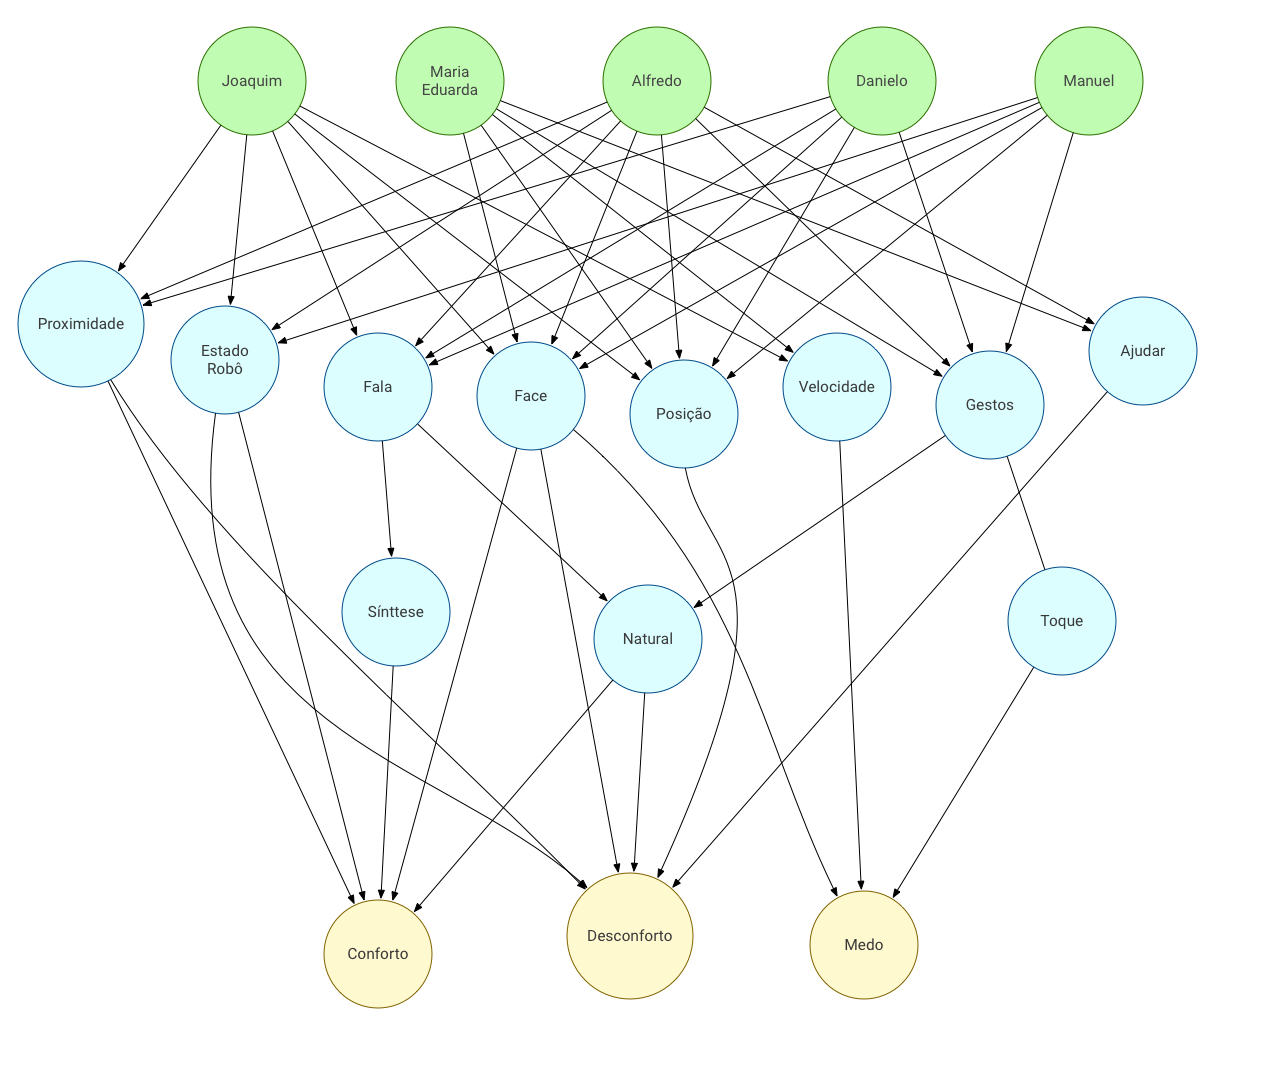
\includegraphics[width=\textwidth]{rb-thesis.png}
		\smallcaption{Fonte: Autor.}
		\label{fig:rb}
	\end{minipage}
\end{figure}

A rede Bayesiana da figura~\ref{fig:rb} funciona da seguinte maneira, são fixados os valores de evidência nos nós evidências (amarelos) e nos nós internos (azuis). Com base nas evidências apresentadas, a rede responde a probabilidade de ser cada uma das Personas que compõem os nós raízes (verdes). A partir da classificação é possível identificar qual o perfil do usuário, em interação com o robô. É importante ressaltar que a classificação do usuário é feita com base em sua experiência, pois é o principal interessado na interação com o robô. A grande preocupação em manter o foco no ser humano é por que ele é o mais interessado na interação com o sistema. A tomada de decisão para melhorar a experiência do usuário a partir da classificação do perfil do usuário pelo robô não faz parte do escopo desta tese. Porém nas seções a seguir são apresentados os passos para definir os valores de probabilidades condicionais, consumir, extrair conhecimento e evoluir o classificador a partir da base apresentada nessa seção.

\subsection{Definindo os valores de probabilidades condicionais}
\label{sec:tpc}
Com a estrutura da rede Bayesiana definida, antes de utilizá-la para classificar as Personas, é necessário definir as tabelas com os valores das probabilidades condicionais para cada variável. Para construir as tabelas de probabilidades condicionais~(TPC), é feito a análise das respostas nos questionários e sobre as anotações realizados durante o teste de interação. Durante o processo de análise é identificado a frequência dos eventos que envolvem cada variável. Nesse momento conseguimos estipular o valor de cada uma das variáveis, como por exemplo, a Persona Danielo representa 1 participante de 39 no total. Sendo assim, a probabilidade de ser ele é de 2,56\%. O seu complemento deve somar uma probabilidade total de 100\%. No caso a probabilidade de não ser a Persona Danielo é de 97,44\%. Para nós sem dependência condicional, como no caso das Personas, esse cálculo é mais concreto. Contudo, quando mais profundo o nó na rede Bayesiana, e mais condicionado a outras variáveis, o cálculo para conseguir definir as probabilidades em 100\% torna-se mais complicado de atingir.

 Então, a partir da contabilidade dos eventos utilizam-se as equações de teoria de probabilidade definidas para encontrar os valores de cada um dos domínios da variáveis da rede Bayesiana. Todos os valores devem ser normalizados para manter a somatória das probabilidades igual a 1, ou seja, igual a 100\%. A partir do cálculo é possível determinar os valores de consultas e utilizar a rede Bayesiana para sua classificação. Dependendo da frequência encontrada, após a normalização a diferença pode ser pequena, principalmente pelo número de variáveis condicionais existentes. Esse problema pode ser solucionado através de mais experimentos e um refinamento da TPC. Os valores de probabilidades condicionais de cada variável são apresentados no apêndice~\ref{ap:tpc} dessa tese. Na sequência, o processo de consumo da rede Bayesiana é descrito para auxiliar na classificação do perfil do usuário como Persona.

\subsection{Executando a classificação da Persona}
\label{sec:consumo}
Para classificar a Persona, é necessário implementar o cálculo das probabilidades condicionais no robô. Com a implementação concluída é realizado a interação do robô, onde é capturado as evidências das variáveis que auxiliam a determinar os valores de cada variável da camada interna e também da camada de evidência da rede Bayesiana.

O resultado a partir das evidências identificadas durante a interação, é a probabilidade de cada Persona ser enquadrada pelo perfil daquele usuário. Para definir a Persona, deve-se identificar qual delas têm a maior probabilidade de ser classificada como similar ao perfil do usuário. Nessa tese, para efeito de visualização da rede Bayesiana, utilizou-se um programa chamado SamIam~\footnote{http://reasoning.cs.ucla.edu/samiam/}. Ele é capaz de criar e executar uma rede Bayesiana através de uma interface visual, facilitando identificar o comportamento dela. A figura~\ref{fig:samiam} apresenta a interface do programa SamIam.

\begin{figure}[ht!]
	\centering
	\begin{minipage}{\textwidth}
		\caption{Rede bayesiana implementada no programa SamIam.}
		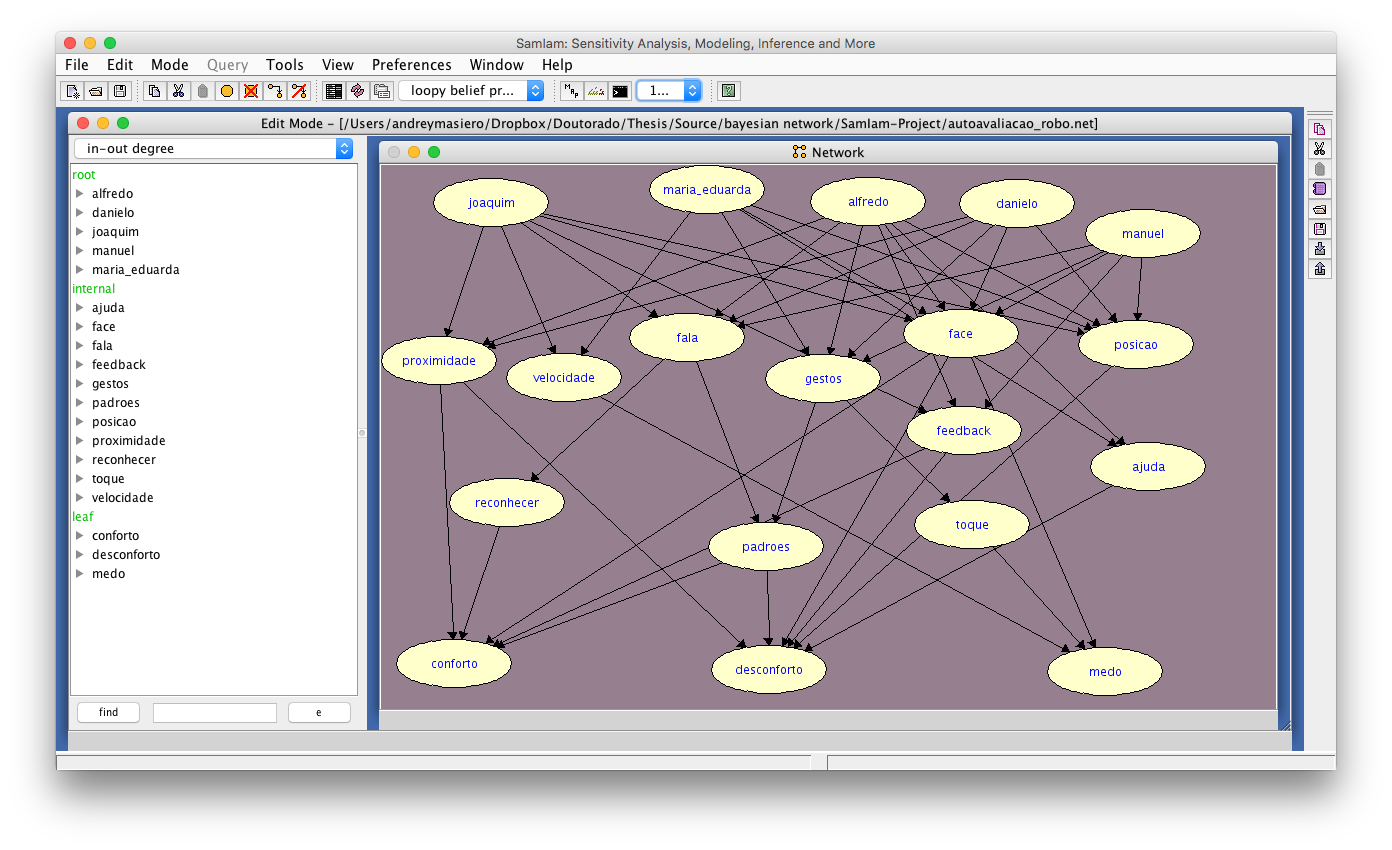
\includegraphics[width=\textwidth]{samiam.png}
		\smallcaption{Fonte: Autor.}
		\label{fig:samiam}
	\end{minipage}
\end{figure}

Na figura~\ref{fig:samiam} é apresentado a implementação da rede Bayesiana estrutura na figura~\ref{fig:rb}. Nele é possível monitorar as variáveis que representam as Personas e, ao alterar os valores das variáveis de evidência e saber qual o perfil com maior probabilidade. As análises e detalhes sobre os testes são discutidos no capítulo~\ref{cap:resultados}.